\documentclass{aamas2013}

\usepackage{cancel}
\usepackage{subfigure}
\usepackage{algorithm}
\usepackage{algpseudocode}
\usepackage{times}

\pdfpagewidth=8.5truein \pdfpageheight=11truein

\newtheorem{theorem}{Theorem}
\newtheorem{definition}{Definition}
\newtheorem{corollary}{Corollary}
\newtheorem{lemma}{Lemma}
\newtheorem{proposition}{Proposition}

\begin{document}

\title{Optimal Internet Auctions with Costly Communication}

\numberofauthors{2}

\author{ 
\alignauthor
Yuqian Li\\
	\affaddr{Department of Computer Science, Duke University}\\
	\affaddr{Durham, NC 27708 USA}\\
	\email{yuqian@cs.duke.edu}
\alignauthor
Vincent Conitzer\\
	\affaddr{Department of Computer Science, Duke University}\\
	\affaddr{Durham, NC 27708 USA}\\
	\email{conitzer@cs.duke.edu}
}


\maketitle

\begin{abstract}
Iterative auctions can reach an outcome before all bidders have 
revealed all their preference information.  This can decrease costs
associated with communication, deliberation, and loss of privacy.
We propose an explicit cost model that is inspired by single-item
Internet auctions, such as those taking place on auction sites (eBay)
or via informal communication (craigslist, mailing lists). 
A nonzero bid comes at a cost to both the seller and the bidder, and
the seller can send broadcast queries at a cost.
Under this model, we study auctions that maximize the seller's profit 
(revenue minus seller cost).
We consider multi-round Vickrey auctions (MVAs), in which the seller
runs multiple Vickrey auctions, with decreasing reserve prices.
We prove that restricting attention to this class is without loss of
optimality, show how to compute an optimal MVA, and compare
experimentally to some other natural MVAs.
Among our findings are that (1) the expected total cost is bounded
by a constant for arbitrarily many bidders, and (2) the optimal MVA
and profit remain
the same as long as the total bid cost is fixed, regardless of which
portion of it belongs to the seller and which to the buyer.
\end{abstract}

\category{I.2.11}{Artificial Intelligence}{Distributed Artificial
Intelligence}[Multi-agent systems]
\category{J.4}{Social and Behavioral Sciences}{Economics}

\terms{Algorithms, Economics, Theory}

\keywords{Auctions, mechanism design, communication costs}

\section{Introduction}

Auctions constitute a favored method for allocating scarce resources in
multiagent systems.  However, communication requirements can pose a
bottleneck.  Motivated by the revelation principle, much of the theory of
mechanism design considers {\em direct-revelation} mechanisms, in which
each agent declares its entire valuation function to the auctioneer.  The
corresponding overhead, not only in terms of communication per se but also
in terms of the agent having to completely {\em determine} its valuation
function, can be prohibitive.  All of this is well understood (for further
discussion, see, e.g.,~\cite{Conitzer04:Computational}), and a significant amount of research has been
devoted to the design of {\em iterative} auction mechanisms (e.g.,~\cite{Parkes06:Iterative}) and (roughly
equivalently) auctions with explicit {\em elicitation} of agents'
valuations (e.g.,~\cite{Sandholm06:Preference}).  Such auctions aim to avoid
unnecessary communication.  For example, in a Vickrey auction, if it is known
that bidders 1 and 2 have valuations above \$100 and bidder 3 has one below
\$100, then there is no need to query bidder 3 any further.

How do we evaluate how effective a particular iterative auction mechanism
is in reducing communication?  Perhaps the simplest measure is the number
of bits communicated (see, e.g.,~\cite{Nisan05:Communication}).  Within a particular query
model, it may also make sense to minimize the total number of queries (see,
e.g.,~\cite{Lahaie04:Applying}). However, in this paper, we argue that such existing models
fail to capture important aspects of the cost of communication in certain
types of Internet auctions.  In particular, in such auctions often the most
costly communication that takes place is the {\em first} time that a bidder
gives a positive response, indicating having a nonzero value for an item.
This can be the case for several reasons.  One possibility is that the
auction website at this point may insist that the bidder provides payment
(say, credit card) information or places money in escrow.  Otherwise, a
malicious user may steer the auction in a particular direction and in the
end refuse to pay.  Alternatively, in other settings (such as an item
having been posted for sale on craigslist or a similar list), at this point
the bidder may wish to set up an appointment with the seller to check the
item.  In both cases, these actions come at costs for both the potential
buyer and the seller, in terms of effort, time, loss of privacy, and 
so on.
%The bidding costs $c$ may be caused by communication and other verification
%required to bid. For example, the bidder may have to input his credit card
%number and prepay an amount of money. Without such verification, a bidder may
%bid very high and refuse to pay in the end. 
%A verification for the seller might
%also be needed. For example, a bidder may want to set up an appointment with
%the seller to check the item.  Setting up such an appointment might be costly
%because they need to dicuss time and place via emails or phone calls.
%Attending that appointment may also cost travel fees and time.  
While participation costs have been studied before in
%Note that our
%bidding cost is different from conventional participation cost studied before
auctions~\cite{Stegeman95:ParticipationCost,
  Tan2006:EquilibriaParticipationCost}, a distinguishing feature of our
model is that a bidder can observe the proceedings of the auction at no
cost, until the bidder decides to actively participate by indicating a
nonzero valuation and thereby changing the course of the auction.   This
appears to us to be a more natural model of Internet (or other highly
anonymous) auctions of the type discussed above.
%In
%our model, it is free for bidders to participate without bidding, which is more
%close to most Internet platforms. In another word, bidders do not have to buy a
%ticket to walk in and observe.

The rest of this paper is organized as follows.  In Section~\ref{sec:model}, we
provide a formal model of communication cost motivated by the observations just
discussed.  In Section~\ref{sec:efficient}, we study the special case in which
efficient allocation is a constraint and bidders experience no cost from
bidding.  The characterization of the optimal mechanism in this special case
turns out to be closely related to earlier work on finding an optimal agent by
iteratively relaxing the parameters of the search
~\cite{SarneSR2010:IncreasingSearch} (see more detailed discussion at
the end of Section \ref{sec:alpha-MVA}).  In Section~\ref{sec:general}, we drop
the assumptions of efficiency and no bidder cost for communication. In both
cases, the optimal auctions are proved to be multi-round Vickrey auctions (MVAs),
which were previously studied by \cite{McAfee97:SequentialAuctions}, but with a
different motivation, time discount, rather than communication cost. 


%\subsection{Related research}






\section{Cost Model and Settings}

In this section, we define our cost model and explain why it makes sense. Our
cost model is inspired from online second-hand item transactions, including
examples like eBay, craigslist and universities' mailing-lists.


\begin{definition}\label{def:model}

In our settings, there's one seller selling one item to $n$ buyers (bidders)
whose valuations $v_i~(1 \leq i \leq n)$ are independently and identically
distributed (i.i.d.) over $[0, 1]$ with PDF $f(x)$ and CDF $F(x)$. The seller
can broadcast a message to all bidders which costs $b$ (the broadcast cost) for
the seller.  A bidder may reply to that broadcast with cost $c$ (bidding cost)
or remain silent with no cost. Such bidding cost $c$ may contain two parts,
$\beta_1, \beta_2$ where $\beta_1+\beta_2 = c$.  The first part $\beta_1$ is
charged to the seller while the second is charged to the corresponding bidder.
The bidder's reply should be deterministic with respect to the seller's
broadcast (for simplicity, we only consider pure strategy equilibrium).

\end{definition}

Most settings in definition \ref{def:model} are quite standard except for the
cost and broadcast capability.

The bidding costs $c$ may be caused by communication and other verification
actions required to put a bidding. For example, the bidder may have to input
his credit card number and prepay an amount of money. Without such verification
for the bidder, a bidder may bid very high and refuse to pay in the end. A
verification for the seller might also be needed. For example, a bidder may
want to set up an appointment with the seller to check the item.  Setting up
such an appointment might be costly because they need to dicuss time and place
via emails or phone calls.  Attending that appointment may also cost travel
fees and time. 

We introduce broadcast capability because it's shared by many auctions.  For
example, a Vickrey auction or a first-price auction with reserve price can be
described as a broadcast auction with only one broadcast: telling every bidder
the reserve price. The bisection auction [cite bisection auctions] is another
example which has many rounds of broadcasts. In each round , it will broadcast
a price and ask bidders to reply whether his valuation is beyond or below that
price.  In real world, sellers make such broadcasts via sending emails to a
bunch of receivers (typically a mailing-list), listing items on a platform such
as craigslist and eBay, or even showing ads on Internet/TV. Such broadcast
activities costs either money (e.g. a list or ads fee) or time and effort (e.g.
writing and sending an email).

Note that in our model, we only give sellers broadcast capability so they
cannot find or communicate with each bidder one by one. The first reason to
have this constraint is there are too many potential bidders on the Internet
(our model focus on online item transactions) and it's hard to explicitly find
them one by one. On the other hand, in offline cases where the set of bidders
are small and explicit (e.g. the government want to sell a land to one of three
companies), it might be helpful to let the seller communicate with bidders one
by one [cite search mechanisms]. The second reason to have this constraint is
that we want to focus on mechanisms that avoids time consuming bargaining. Such
feature is very important as one of the most vital advantages of online
transactions are their convenience and the time consuming bargainning can ruin
it.

Finally, we define optimal mechanisms to be the ones that maximze seller's
utility since when facing many different auction mechanisms, a rational seller
will choose the one that gives him maximum utility.

\begin{definition}

We say a mechanism is optimal if it gives the seller maximum utility (revenue)
which equals to all the value payed to this seller minus all the cost charged
to this seller. A class of mechanisms are optimal if they contain one optimal
mechanism.

\end{definition}


\section{Optimal Mechanisms with Efficiency and Only Seller's Cost}
\label{sec:efficient}

In this section, we make two simplifying assumptions: (1) we restrict
attention to mechanisms that allocate the item efficiently and (2) we
assume that the bidder cost for replying ($\beta_2$) is zero.\footnote{Note
that if (2) does not hold, then allocating efficiently may not be possible
without the seller compensating the bidders for their bid costs.}
%we consider a simplified optimizing problem with efficiency
%constraint and only seller's cost.  Though these two constraints simplify our
%problem a lot, they are reasonable in real cases such as craigslist or moving
%sales in mailing-lists. 
For example, someone who is moving and selling furniture on craigslist is
likely to have $0$ valuation for the item 
and cannot commit to withhold the item or prevent re-sale between
bidders. Under such circumstances,  efficient mechanisms not only maximizes the
social welfare but also maximizes the seller's revenue
\cite{Ausubel99:EfficientOptimality} (though this does not consider
communication costs).
% Besides, every bidder would at most be
%charged for one bidding but the seller will be charged for all
%biddings. Thus it also seems reasonable to ignore bidder's bid cost
%for simplicity.
In Section~\ref{sec:general} we drop these assumptions.


%\begin{enumerate}
%
%\item In many cases, sellers only have $0$ valuation for the item.
%For example, some second-hand items will be tossed if they cannot be sold by a
%particular day, e.g. the day the seller moves out the house. We encounter many
%free items during second-hand sales as well, which is another demonstration of
%zero valuation. Additionally, sellers cannot commit to withhold the item or 
%prevent re-sales between buyers. Under such circumstances, an efficient mechanism not only
%maximzes the social welfare but also maximizes the seller's revenue \cite{Ausubel99:EfficientOptimality}.
%
%\item The bid cost for each bidder sometimes seems \footnote{But actually
%it is not that negligible as our example seems to claim. In later section,
%theorem \ref{theorem:equivalence} will show exactly how important it is.} to be
%negligible compared to bid cost charged to the seller. For example, if
%$100$ bidders replied to the seller by a $1$-minue call, each bidder only has a
%tiny $1$ minue cost.  But for the seller, it is a big $100$ minutes cost which
%is very annoying. It is also necessary to remove bidder's bid cost to
%achieve efficiency (without compensation).  Otherwise, the item may not be able
%to allocate to the highest bidder when that highest valuation is below the
%bidder's bid cost.
%
%\end{enumerate}

The rest of this section is organized as follows. First, we
introduce a class of mechanisms called multi-round Vickrey auctions (MVA).
%based on
%what has been used in realworld online second-hand item transactions.  
Then,
we prove that we can restrict attention to MVAs without loss of optimality.
%(so there exists a MVA that is
%optimal). A
After that, we find the specific MVA that is optimal. Finally, we
experimentally compare this optimal MVA to some other natural mechanisms.

\subsection{Multi-round Vickrey Auctions}


In an MVA, the seller runs a Vickrey auction with a reserve price; if
nobody bids (above the reserve price), the seller runs another Vickrey
auction with a lower reserve price, etc., until the item is sold.  (In
Section~\ref{sec:general}, we will also consider MVAs that can terminate
without having sold the item.)
%n MVA has multiple rounds of Vickrey
%auctions with progressively decreasing reserve prices. 
For example, consider a sequence of eBay auctions (with proxy bidding) in
which the seller is repeatedly lowering the reserve price.


%This kind of auction
%effectively occurs on eBay. The seller may set up a reserve price and let
%buyers bid for this item. The proxy bidding functionality makes such an auction
%equivalent to a Vickrey auction with a reserve price. If no buyers bid for a
%given reserve price, the seller may lower the reserve price, which makes the
%whole process equivalent to an MVA.

\begin{definition}[Multi-round Vickrey Auction (MVA)]
  An MVA is defined by a sequence of reserve prices $r_1, r_2, \ldots$
  (which may be finite or infinite) where $r_i > r_{i+1}$. In round $i$, a
  Vickrey auction with reserve price $r_i$ is run (if the item has not been
  sold).
%The seller creates a Vickrey
%auction with a reserve price $r_i$ at time $i$ (or round $i$). In each
%Vickrey auction, if only one buyer bids, he/she gets the item and pays reserve
%price. Otherwise, the buyer with the highest bidding gets the item and pays the
%second highest bidding.
\end{definition}

%MVAs require Vickrey auctions (or equivalent English auctions) as basic steps.
%In reality, however, such functionality won't always be provided by online
%platforms such as craigslist. Thus a simplified version of MVA occur very often
%in those platforms. People call it first-come first served which means for
%every reserve price $r_i$, the first one who accept that price wins the item
%and pays $r_i$ directly. This mechanism may loose revenue and social efficiency
%as the person with lower valuation $p$ may get the item for $r_i$ while there's
%someone else who is willing to pay a higher amount of $q$ where $r_i \leq p < q
%< r_{i-1}$. We won't focus on this first-come first served mechanism because
%it's harder to analyze analytically and it's inferior than MVAs in terms of
%both sellers' utility and social welfare.

%Since there is no cost charged to buyers, 
In an MVA, {\em if} a bidder decides to bid (above the reserve price), it
is optimal to bid truthfully since doing so is dominant in a Vickrey auction.
However, a bidder may choose strategically to stay silent even with a
valuation above the reserve price, in the belief that nobody else will bid this
round so that the price will decrease in the next round.
%it is obvious to see that whenever a
%bidder decides to bid, he/she must bid truthfully. 
%vc: could make this a proposition...  not clear it's worth it.  is there a
%reference? mcafee and vincent?
Thus, in our (symmetric) setting, Bayes-Nash
Equilibria (BNE)
 for MVAs can be described by a sequence of thresholds $a_1, a_2,
\ldots$ where $a_i > a_{i+1}$; in round $i$, a bidder bids if and only
if his valuation is at least $a_i$.
%Whenever a bidder's valuation for the item
%is greater than $a_i$, he/she is going to bid in round $i$ whose reserve price
%is $r_i$. 


We will be interested in the following question: given desired thresholds
$a_i$, which reserve prices $r_i$ result in these thresholds?  Then, by the
revelation principle, we can convert this to a mechanism in which we query
agents whether their valuations are above $a_i$ and it is optimal for them
to respond truthfully.

%In later analysis, we firstly decide thresholds $a_i$ since they are more
%meaningful for bidders to make decisions and for us to make analysis. Then we
%determine the right reserve prices $r_i$ that make bidders incentive compatible
%to bid according to thresholds $a_i$. 

\begin{lemma}
  Consider a symmetric strategy profile in an MVA where in the $i$th round,
  valuation $a_i$ is the threshold for bidding (so that bidders with lower
  valuations stay silent and those with higher valuations bid).  Then this
  constitutes a Bayes-Nash equilibrium if:
\begin{align}\label{eq:MVA_eq}
%    &r_k = a_k = 0 \mbox{ and }
    %&\forall i, i+1\nonumber\\% ~(1 \leq i < k),\nonumber\\
    &~~P(a_{i})(a_{i}-r_i) =
    \int_{a_{i+1}}^{a_{i}}(a_{i}-x)p(x)dx+P(a_{i+1})(a_{i}-r_{i+1})
\end{align}
(where 
%\begin{align*}
$P(x) := F(x)^{n-1}$ and $p(x) := P'(x) = (n-1)F(x)^{n-2} f(x)$)
%\end{align*}
when $i$ is not the last round, and either $a_i=r_i$ when $i$ is the last
round or $\lim_{i \rightarrow \infty} a_i = \lim_{i \rightarrow \infty}
r_i$.
\label{lemma:sufficient}
\end{lemma}
\begin{proof}
  Consider a bidder with valuation $a_i$; we first show that in round $i$,
  such a bidder is indifferent between bidding and staying silent if the
  condition holds.  If $i$ is the last round, clearly he is indifferent
  between bidding and not iff $a_i=r_i$.  We now consider the case where
  $i$ is not the last round.  If another bidder bids in round $i$, that
  bidder will bid at least $a_i$, and our bidder will have zero utility.
  Therefore, the left-hand side of (\ref{eq:MVA_eq}) represents the
  expected utility to our bidder for bidding now.  Corresponding to the
  right-hand side, if our bidder stays silent, and there is a next round
  and our bidder bids in that next round, then he will win in that round,
  either with another bidder bidding (first term) or not (second term).

  If we now consider a bidder with valuation above $a_i$, a similar
  analysis shows that this bidder strictly prefers bidding in round $i$ to
  waiting one more round; inductively, he will prefer it to waiting any
  number $k > 0$ more rounds; and he will also prefer this to never bidding
  because either $a_j=r_j$ when $j$ is the last round or $\lim_{j
    \rightarrow \infty} a_j = \lim_{j \rightarrow \infty} r_j$.   Finally,
  let us consider a bidder whose valuation lies below all the $a_i$.
  Because either $a_j=r_j$ when $j$ is the last round or $\lim_{j
    \rightarrow \infty} a_j = \lim_{j \rightarrow \infty} r_j$, this bidder
  is best off never bidding.
\end{proof}

%The equation \ref{eq:MVA_eq} says that the bidder with valuation $a_i$ should be
%indifferent from bidding in round $i$ (the left hand side) or bidding in round
%$i+1$(the right hand side).  The following theorem describes the equilibrium of
%MVAs determined by equations above.

For a mechanism that allocates efficiently, we either have $r_k = a_k = 0$
for some $k$, or $\lim_{i \rightarrow \infty} r_i = 0$.

\begin{theorem}
Given a decreasing sequence of $a_i \in [0,1)$ that ends at or converges to
$0$, let
\begin{align}\label{eq:MVA_eq_relation}
%  r_k &= a_k = 0 \nonumber \\
  r_i &= \left( \int_{0}^{a_i} x \, p(x) dx \right) / P(a_i) & (\mbox{if $a_i > 0$})
\end{align}
and $r_i=0$ if $a_i=0$. The corresponding MVA has a pure strategy Bayes-Nash equilibrium characterized by
bidding thresholds $a_1, a_2, \ldots$.
%. where the bidder with valuation at least $a_i$
%but less than $a_{i-1}$ (presumably $a_0 = 1$) will bid in round $i$ 
\end{theorem}

\begin{proof}
We show that the conditions of Lemma~\ref{lemma:sufficient} hold.  If $i$
is the last round, then $a_i=0=r_i$.  Also, $$\lim_{i\rightarrow\infty} r_i \leq \lim_{i\rightarrow\infty}
\left( \int_{0}^{a_i} a_i \, p(x) dx \right) / P(a_i) = \lim_{i\rightarrow\infty} a_i = 0$$
If $i$ is not the last round, 
by (\ref{eq:MVA_eq_relation}) we have $r_i P(a_i) = \int_{0}^{a_i}
x\,p(x)dx$ for all $i$ (this clearly also holds if
$a_i = 0$). Thus the right-hand side of Equation (\ref{eq:MVA_eq}) is:
\begin{align*}
	& \int_{a_{i+1}}^{a_i} a_i p(x) dx - \int_{a_{i+1}}^{a_i} x \, p(x) dx + P(a_{i+1})(a_i-r_{i+1}) \\
	&= a_i P(a_i) - \cancel{a_i P(a_{i+1})} - r_i P(a_i) + \cancel{r_{i+1} P(a_{i+1})} \\
		& ~~~ + \cancel{P(a_{i+1}) a_i} - \cancel{P(a_{i+1}) r_{i+1}}
%	&= \mbox{left hand side of (\ref{eq:MVA_eq})}
\end{align*}
which equals to left-hand side.
\end{proof}
%vc: think about the inefficient allocation case?

This tells us that a bidder will bid in a round of an MVA if and only if
the expected second-highest bid conditional on this bidder's valuation
being the highest is greater than the reserve price of that round. For
example, if the distribution is uniform, $r_i = \frac{n-1}{n}
a_i$. 

A similar analysis to the one in this subsection (in a model that
includes discounting) appears in~\cite{McAfee97:SequentialAuctions}.  
However, that paper does not consider communication costs, and so we
diverge from that work in what follows.
%has given some more discussions
%and proof (e.g. once a bidder choose to bid, bid truthfully is a unique
%weekly dominant strategy) about the equilibrium of this kind of sequential
%auctions.  That paper, however, aims on the optimal auctions for a
%different cost model with time discount but without broadcast or bidding
%cost. We will discuss this difference later when we introduces bid cost
%for bidders.

\subsection{Optimality of MVAs}


%Done vc: need to add no-gap assumption from revenue equivalence to model
%(anything else?)
Since the mechanism is required to be efficient and bidders' communications
costs ($\beta_2$) are zero, any mechanism that gives utility zero to an
agent with valuation zero results in the same revenue for the seller, by
the revenue equivalence theorem~\cite{Myerson:1981}.\footnote{Moreover, by
  individual rationality we cannot give an agent with valuation zero less
  than zero utility; we could give such an agent more than zero utility (as
  in redistribution mechanisms~\cite{}), but this would only hurt revenue.}
Hence, maximizing profit is equivalent to minimizing the seller's query
costs.

By the revelation principle, we can restrict our attention to mechanisms in
which agents always answer truthfully in equilibrium.\footnote{For
  example, for MVAs, we can directly query the agents whether their
  valuations are above $a_i$ while still charging according to 
  $r_i$.}  By Proposition~\ref{prop:sufficient}, we can assume that an
agent reveals his entire valuation when not staying silent.  By the
efficiency constraint, the mechanism must at least discover a bidder with
the highest valuation.  This optimization problem corresponds to
Definition~\ref{def:query}. 

%he best case is that every reply contains the exact
%and truthful valuation of the corresponding bidder since every reply (or
%bidding) has a cost $c$. By doing that, we never need someone to reply twice.
%The optimizing problem in this best case is defined as definition
%\ref{def:query}.  This best case minimum cost provides us a lower bound for
%minimum cost of our mechanisms. We will then prove that MVAs can achieve this
%lower bound so they are optimal.

\begin{definition}\label{def:query}
  A {\em (direct-revelation) query} is given by a subset $Q \subseteq
  [0,1)$, such that if the agent's valuation is in $Q$, he replies with his
  exact valuation, and otherwise stays silent.  
  %The cost of a query is $b+j
%  \cdot c$ where $j$ is the number of bidders who do not stay silent. 
A strategy for asking queries can be represented by a function
\begin{displaymath}
	S\big(f, m, V, \mathcal Q = \{Q_1, Q_2, \ldots, Q_{i-1} \}\big) = Q_i
\end{displaymath}
which means: 
suppose that the set of queries asked previously is
$\mathcal Q$, the set of values already reported is $V$, and there are $m$
bidders left who have not responded (whose valuations were drawn
i.i.d.~from $f$); then the strategy $S$ will next ask $Q_i$.
We will use $Q_i = \emptyset$ as shorthand for terminating the algorithm.
%suppose there are still $m$ i.i.d.unknown values left whose PDF
%is $f(x)$, the reported values set is $V$ and the set of queries asked is
%$\mathcal Q$, the strategy $S$ will make $Q_i$ as the next query.
%Assume there are $n$ values $v_i ~(1 \leq i \leq n)$ independently and
%identically distributed over $[0, 1)$ with PDF $f(x)$ and CDF $F(x)$.  A query
%strategy is to find the maximum value by asking queries $Q_1, Q_2, \ldots$
%sequentially where $Q_i \subset [0, 1)$ and $\forall i \neq j, ~Q_i \cap Q_j =
%\emptyset$.  After a query $Q_i$, all numbers within $Q_i$ will be reported.
%Note that $Q_i$ may depend on results of $Q_1$ to $Q_{i-1}$. Thus a
%strategy can be denoted as a function:
%\begin{displaymath}
%	S\big(f, m, V, \mathcal Q = \{Q_1, Q_2, \ldots, Q_{i-1} \}\big) = Q_i
%\end{displaymath}
%which means, suppose there are still $m$ i.i.d. unknown values left whose PDF
%is $f(x)$, the reported values set is $V$ and the set of queries asked is
%$\mathcal Q$, the strategy $S$ will make $Q_i$ as the next query.
%The cost of each query is equal to $b+j \cdot c$ where $j$ is the number of
%reported values from that query. 
$C_{f,n}(S)$ is the expected cost of strategy $S$, and we wish to find
$C_{f,n}^* = \inf_S C_{f,n}(S)$.
%The cost of a strategy for a given set of
%unknown values $v_i$ is equal to the sum of all queries' costs it has to make
%before identifying the maximum value. The optimal query strategy is the one
%that has minimum expected cost.  We will write such minimum expected cost as
%$C^*(f, n)$, a function of PDF $f(x)$ and number of unknown values in the
%beginning $n$.
\end{definition}

To find out the optimal query strategy, we first show that the minimum cost
is independent of the PDF $f(x)$.

\begin{lemma}\label{lemma:uniform}
Consider the uniform PDF $f_u(x) = 1$ and let $C^*_n = C^*_{f_u, n}$.
For any other PDF $f(x)$, we have $C^*_{f, n} =  C^*_n$.
\end{lemma}

%Done vc: inconsistency -- subscript or argument of the function?

\begin{proof}
%Let $F^{-1}(x) = \sup\{y ~|~ F(y) = x\}$. 
For any strategy $S_{f_u}$ for the uniform distribution, we can transform
it into a strategy $S_f$ for the distribution  with PDF $f$ 
by querying at the equivalent percentiles. Specifically, 

$
S_f\big(f, m, V, \mathcal Q \big) = F^{-1}\Big( S_{f_u}\big( f_u, m, F(V), F (\mathcal Q) \big) \Big)
$

The performance of $S_f$ on $f$ is the same as that of $S_{f_u}$ on $f_u$.
Therefore,  $C^*_{f, n} \leq C^*_{f_u, n}$.
Conversely and similarly, for any strategy $S_f$
for PDF $f$, we can transform it into a strategy $S_{f_u}$ for uniform PDF
$f_u$. Specifically,

$
S_{f_u}\big(f_u, m, V, \mathcal Q \big) = F\Big( S_f\big( f, m, F^{-1}(V), F^{-1} (\mathcal Q) \big) \Big)
$

Thus, $C^*_{f_u, n} \leq C^*_{f, n}$.  Hence,  we have $C^*_{f, n} = C^*_{f_u, n}
= C^*_n$. Figure \ref{fig:uniform} 
illustrates those two constructions we used for this proof.
\end{proof}

%Done vc: update notation in figures below
\begin{figure}
\centering
  \subfigure[Construct $S_{f}$ from $S_{f_u}$]{
    \includegraphics[width=.45\linewidth]{figures/S-u-to-f}
    \label{fig:S-u-to-f}
  }
  \subfigure[Constructing $S_{f_u}$ from $S_f$.]{
    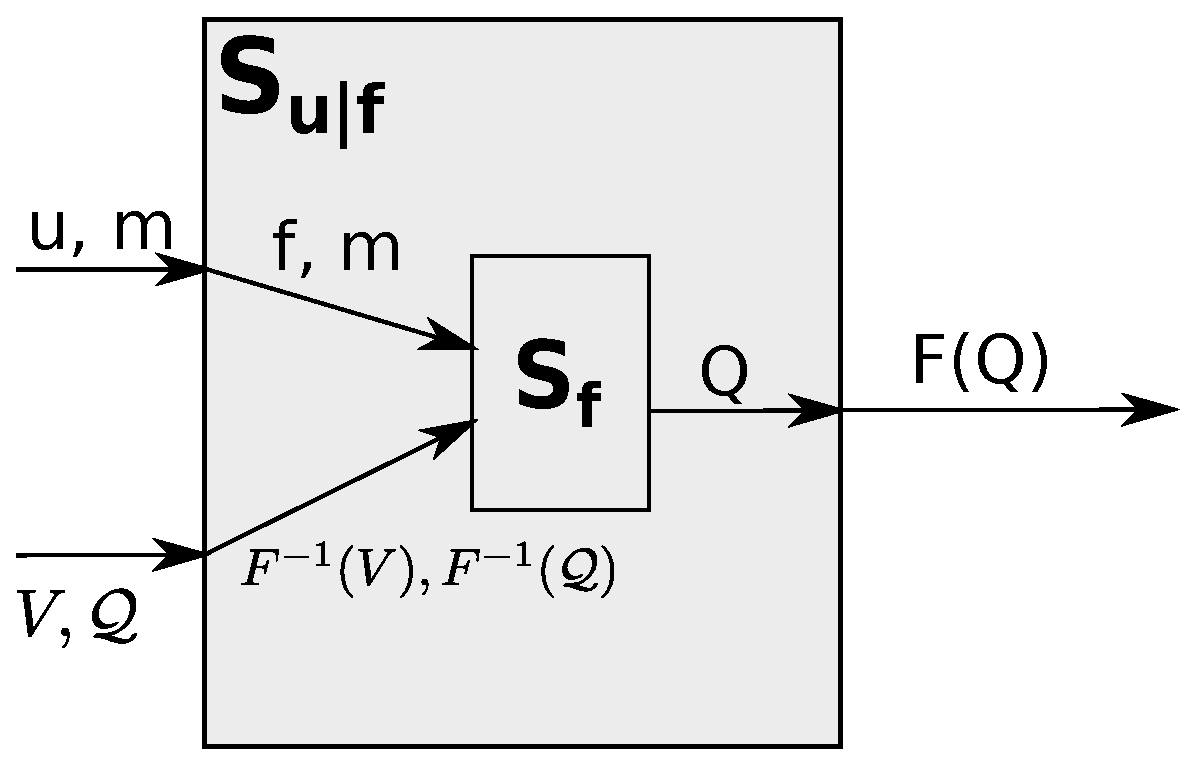
\includegraphics[width=.45\linewidth]{figures/S-f-to-u}
    \label{fig:S-t-to-u}
  }
  \caption{These two figures illustrate how to construct a strategy for an
    arbitrary PDF $f$ from one for the uniform distribution $f_u$, and vice versa.
Here, we depict a strategy as a box that takes four inputs $f, m, V,
  \mathcal Q$ (PDF, number of unknown values, reported values set, and set of asked
  queries) and returns $Q$ (the next query).} \label{fig:uniform}
\end{figure}

We next prove that descending query strategies, in which all bidders are
asked whether their valuations are above $a_i$ for a decreasing sequence of
$a_i$, are optimal.  (For a descending query strategy, as soon as we get a
positive reply, we are done, so the contingency plan does not need to branch.)

\begin{lemma}\label{lemma:descending}
Every optimal strategy 
uses only 
descending queries
$Q_1 = [a_1, 1), ~Q_2 = [a_2, a_1), ~Q_3 = [a_3, a_2)\ldots$
(with the possible exception of strategies that differ only on a measure
zero set
and are therefore equivalent to a descending-query strategy with
probability $1$).
\end{lemma}

\begin{proof}
Let us assume, for the sake of contradiction,
that there exists  an optimal strategy  that uses a 
non-descending query (meaning, one that differs from a descending query on
a non-measure-zero set).
In that strategy $S$, there must be a first non-descending query
$Q_{i+1} = S\big(F, m, V, \mathcal Q = \{Q_1, Q_2, \ldots, Q_i\}\big)$
% where
%$Q_1$ to $Q_i$ are all descending.  
Consider an alternative descending query
$Q'_{i+1} = [a'_{i+1}, a_i)$ (presumably $a_0 = 1$) such
that $|Q'_{i+1}|_f = |Q_{i+1}|_f$
where for any query $Q$, $|Q|_f$ denotes the probability under $f$ of the
region queried by $Q$.
%\[
%\Pr(v \in Q_{i+1}) = \int \limits_{Q_{i+1}} f(x) \mathrm d x = \int \limits_{Q'_{i+1}} f(x) \mathrm d x = \Pr(v \in Q'_{i+1})
%\]
%(After $Q'_{i+1}$, we query optimally.)
%After $Q'_{i+1}$, we will use as optimal query as
%possible.

Because $Q_1$ to $Q_i$ are all descending, we have $m = n$ and $V = \emptyset$ (otherwise
an optimal strategy should terminate without asking $Q_{i+1}$).
Let $C$ be the expected cost of using $S$ from this point on
(starting with $Q_{i+1}$), and let $C'$ be the expected cost of 
of using $Q'_{i+1}$ and querying
optimally after that. We have\\
$
C = b + \sum_{j=0}^n p_j ( j \cdot c + L_j)
$
and
$
C' = b + \sum_{j=0}^n p'_j ( j \cdot c + L'_j)
$
where
%\begin{enumerate}
%\item 
$p_j$ (or $p'_j$) is the probability that there are $j$ reported values
within $Q_{i+1}$ (or $Q'_{i+1}$), and
%\item 
$L_j$ (or $L'_j$) is the expected cost of later queries given that $j$ values have been
found in $Q_{i+1}$ (or $Q'_{i+1}$).
%\end{enumerate}

% yuqian: we have, we have?
Because $|Q'_{i+1}|_f = |Q_{i+1}|_f$,
%\Pr(v \in Q_{i+1}) = \Pr(v \in Q'_{i+1})$
we have $p'_j = p_j$
for all $j$.  We have $L_n = L'_n = 0$.
By Lemma~\ref{lemma:uniform},
$L_0 = L'_0 = C^*_n$ 
because if we know that no value lies in $Q_1, Q_2, \ldots, Q_{i+1}$, the
remaining problem  is equivalent to that with the revised PDF
\[
f_{i+1}(x) = \begin{cases}
	\lambda f(x), & x \notin Q_1 \cup Q_2 \cup \ldots \cup Q_{i+1} \\
	0, & x \in Q_1 \cup Q_2 \cup \ldots \cup Q_{i+1}
\end{cases}
\]
where $\lambda$ is a constant that makes $\int_0^1 f_{i+1}(x) dx = 1$.
Finally, since $Q'_{i+1}$ is a descending query, for all $0 < j < n$,
$L'_j = 0$ but $L_j > 0$ (because for these values of $j$, it is possible
that all reported values in $Q_{i+1}$ lie below some value that has not
been queried yet).  Moreover, there exists some $j$ with $0 < j < n$ and
$p_j > 0$ unless (1) the probability of each agent's reply to $Q_{i+1}$ is
$1$---but in this case it differs only on a measure zero set from the
descending query that asks for all the remaining values, contradicting our
assumption; (2) the probability of each agent's reply to $Q_{i+1}$ is
$0$---but such a measure zero query is clearly suboptimal;
or (3) $n=1$---but in this case any query that differs by more
than a measure zero set from the query that asks for all the remaining
values is clearly suboptimal.
Hence, $C' < C$, contradicting our initial assumption.
\end{proof}

It follows that:

%Done vc: somewhere say something about having to query even when 1 bidder
%remains.  move up no-blind-allocation def and maybe refer to it in theorems

\begin{theorem}\label{theorem:MVA_eq}
Among all mechanisms
that are
required to allocate efficiently,
%(allocate the item to the bidder with highest
%valuation), 
Multi-round Vickrey Auctions (MVAs) are of minimum cost.
\end{theorem}

\begin{proof}
%The best case optimizing problem defined in definition \ref{def:query} provides
%us a lower bound of minimum cost we can achieve by any mechanisms.  
By Lemma~\ref{lemma:descending}, we can restrict our attention to
mechanisms with  descending query strategies
%such lower bound minimum cost can be achieved by
%descending query strategy 
$Q_1 = [a_1, 1], Q_2 = [a_2, a_1)$, $Q_3 = [a_3, a_2) \ldots$.
For any such mechanism, Theorem~\ref{theorem:MVA_eq} tells us how to find reserve prices $r_1, r_2,
\ldots$ such that the corresponding MVA has a Bayes-Nash equilibrium that
is equivalent to this descending-query mechanism.
% any such mechanism is equivalent to the
%Bayes-Nash equilibrium of an MVA
%we are able to design such an MVA
%with reserve prices $r_1, r_2, \ldots$  whose Bayesian Nash Equilibrium
%achieves this best case descending query strategy.  Thus, MVAs are of minimum cost.
\end{proof}

By the revenue equivalence theorem,  we obtain% that MVAs are optimal:

\begin{corollary}
If the bidders have no cost for bidding ($\beta_2=0$), MVAs 
that minimize cost for the seller
are optimal
among mechanisms that allocate efficiently.
%If all broadcast costs and bid costs are charged to sellers, MVAs are
%optimal if efficiency is required.  Such optimal MVA is the one that minimizes
%the overall cost.
\end{corollary}

\subsection{MVAs with Minimum Cost}
\label{sec:alpha-MVA}

\begin{figure*}
\centering
%  \subfigure{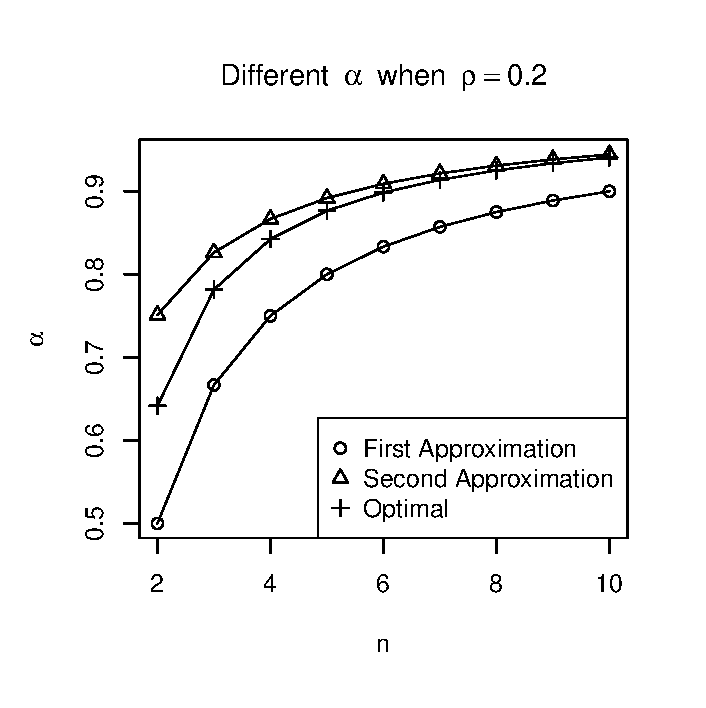
\includegraphics[trim=0 5mm 5mm 5mm, clip, width=.3\linewidth]{figures/alpha_when_rho0.20.eps}}
%  \subfigure{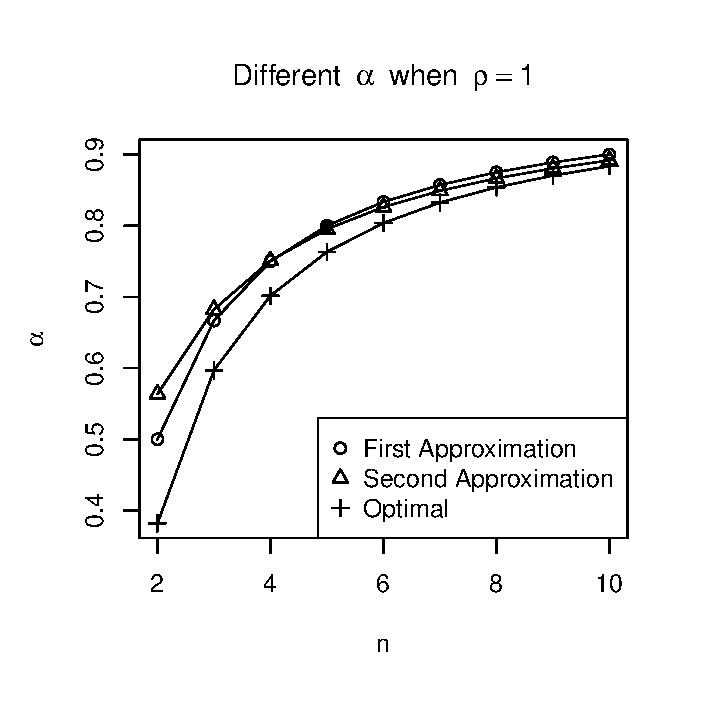
\includegraphics[trim=0 5mm 5mm 5mm, clip, width=.3\linewidth]{figures/alpha_when_rho1.00.eps}}
%  \subfigure{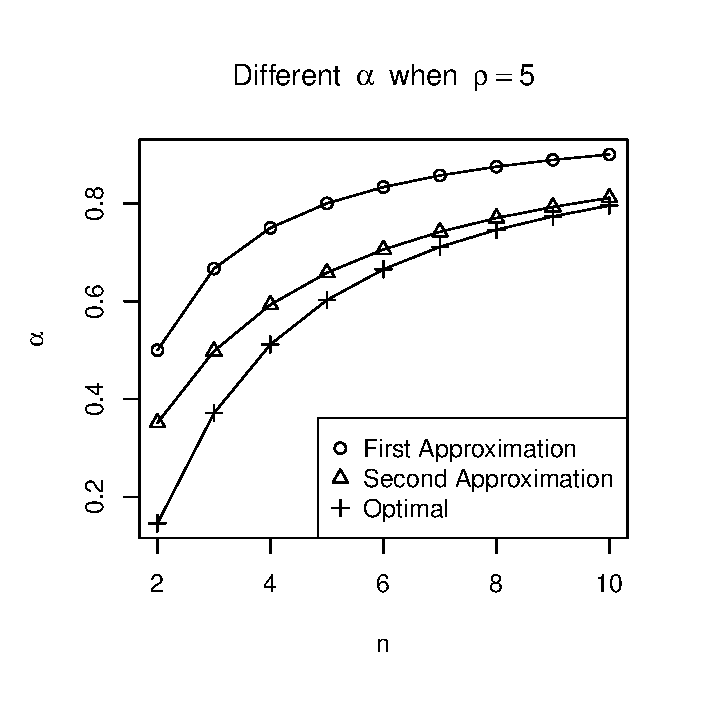
\includegraphics[trim=0 5mm 5mm 5mm, clip, width=.3\linewidth]{figures/alpha_when_rho5.00.eps}}
  \subfigure{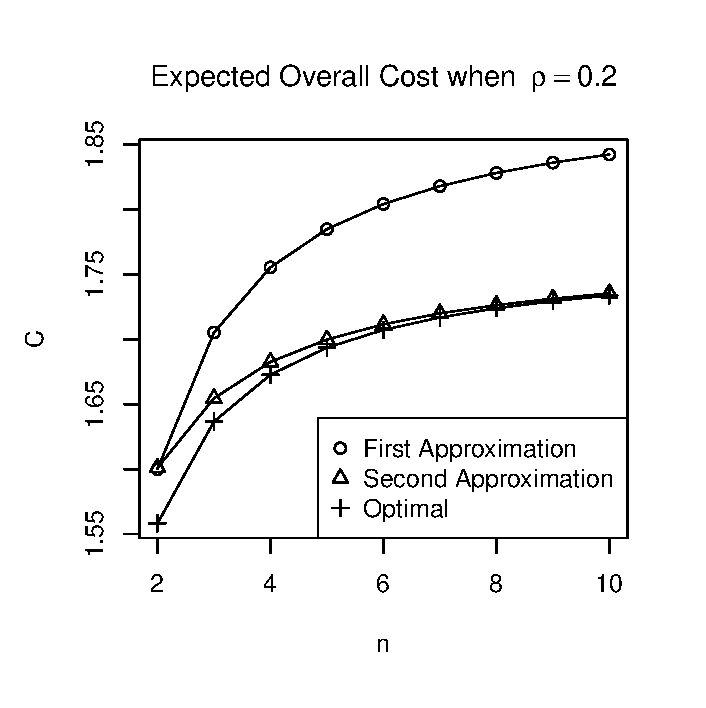
\includegraphics[trim=0 5mm 5mm 5mm, clip, width=.3\linewidth]{figures/C_when_rho0.20.eps}}
  \subfigure{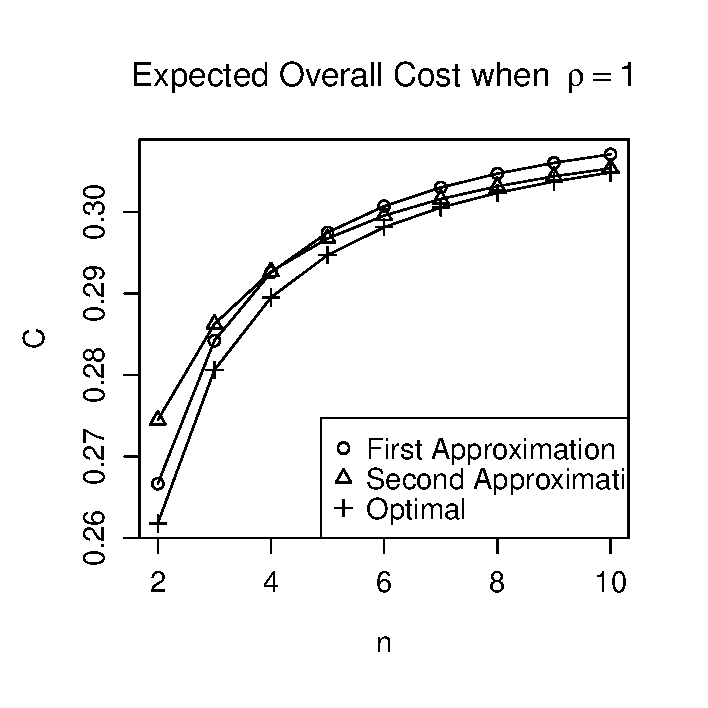
\includegraphics[trim=0 5mm 5mm 5mm, clip, width=.3\linewidth]{figures/C_when_rho1.00.eps}}
  \subfigure{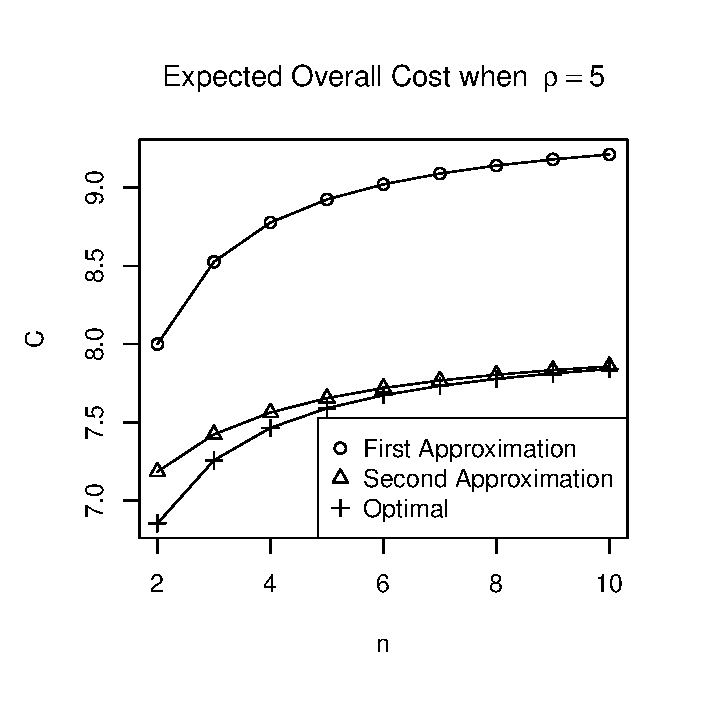
\includegraphics[trim=0 5mm 5mm 5mm, clip, width=.3\linewidth]{figures/C_when_rho5.00.eps}}
  \caption{Comparisons for the optimal $\alpha$ and its approximations. The first
  approximation is $\alpha = 1-1/n$, the second is $\alpha =
  (-W(-1-\rho))^{-1/n}$. ($c = 1, b = \rho$. Recall that $\rho = b/c$~for cases where $c > 0$.)}
%The second row is the corresponding cost for different
%  $\alpha$} 
  \label{fig:alpha}
\end{figure*}

The above analysis still leaves open what the optimal parameters
(thresholds $a_i$, or equivalently, reserve prices $r_i$) of the optimal
MVA are for a given setting $f, n, b, c$ (valuation PDF, number of bidders,
broadcast cost, bid cost).  According to Lemma~\ref{lemma:uniform}, the
cost does not depend on $f$ and it suffices to restrict our attention to
the uniform distribution.
Let $\rho = b/c$ (for cases where $c>0$).

%we can always derive an optimal mechanism for any
%$F$ from a uniform distribution.
% Thus we will focus on uniform cases
%below. 
%We will also introduce $\rho = \frac{b}{c}$ to simplify our analysis
%by normalize bid cost $c$ to $1$ and thus broadcast cost $b$ to $\rho$.

\begin{definition}
Given $f$, we define the $\alpha$-MVA to be the MVA in which, the expected
number of nonsilent bids in each round (conditional on having reached that
round) is $(1-\alpha)n$.  In the case where $f$ is uniform, the
$\alpha$-MVA is characterized by $a_i = \alpha^i$.
\end{definition}

\begin{proposition}
For the purpose of minimizing total cost when $\beta_2=0$ under the constraint of efficient allocation:
If $c = 0$, the Vickrey auction (the $0$-MVA) is optimal.
If $\rho = b = 0$, the Dutch auction (which is approximated by the
$(1-\epsilon)$-MVA) is optimal.  
Otherwise, it is optimal to use an $\alpha$-MVA where $\alpha$ satisfies
\begin{align}\label{eq:alpha}
\alpha^{n-1} (\rho + (1-\alpha)n) - (1-\alpha^n) = 0
\end{align}
%vc: unique solution??
\end{proposition}
\begin{proof}
If $c=0$, the Vickrey auction has cost $b$, which is optimal.
If $\rho=b=0$, the expected total cost of the Dutch auction is $c$ (since
with probability $1$ only one agent will reply), which is optimal.
For the remaining case, we first argue that there must be some $\alpha$-MVA
that is optimal.  
By  Lemma~\ref{lemma:uniform}, we can assume $f$ is uniform.
By Theorem~\ref{theorem:MVA_eq}, some MVA must be
optimal.  For this MVA, consider $a_1$.  If $a_1=0$, this is the
$0$-MVA. If $a_1>0$, then if at least one bidder is above $a_1$, we finish after
the first query; otherwise, the resulting conditional distribution for each
bidder is $f|_{[0,a_1)}$. According to Lemma~\ref{lemma:uniform}, we can
rescale this conditional distribution to the uniform distribution over
$[0,1)$ to arrive back at our original problem; and an optimal mechanism
for that is the same MVA that starts with query $a_1$ (which translates to
$a_1^2$ without rescaling).  Repeated application of this reasoning results
in the $\alpha$-MVA with $\alpha=a_1$.

All that remains to show is the characterization of this $\alpha$.
If $C_\alpha$ is the expected overall cost for the $\alpha$-MVA, then we
have $C_\alpha = b + (1-\alpha)nc + \alpha^n C_\alpha$, or equivalently 
$C_\alpha = \frac{b+(1-\alpha)nc }{ 1-\alpha^n}$.
If we optimize this with respect to $\alpha$, we must either have
\begin{align*}
\frac{\partial C_\alpha}{\partial \alpha} = \frac{{\alpha}^{n-1}\,n\,\left(
b+\left( 1-\alpha\right) \,nc\right) }{{\left( 1-{\alpha}^{n}\right)
}^{2}}-\frac{nc}{1-{\alpha}^{n}} &= 0 \nonumber\\
&\Updownarrow\nonumber\\
\alpha^{n-1} (\rho + (1-\alpha)n) - (1-\alpha^n) &= 0
\end{align*}
%Done vc: double-check first equation (unnormalized)
or have $\alpha$ at a boundary value ($0$ or $1$). However, $\alpha=1$ (or
approaching $1$) is clearly suboptimal unless $b=0$, a case that we have
already covered; $\alpha=0$ can be ruled out as $\frac{\partial
  C_\alpha}{\partial \alpha} |_{\alpha = 0} < 0$.
\end{proof}


%An optimal MVA must be an $\alpha$-MVA where each round only $(1-\alpha) n$
%bidders are expected to bid, i.e. $a_1 = \alpha, a_{i+1} = \alpha \cdot a_i$
%for uniform cases. Then the expected overall cost $C$ satisfies: $ C = \rho +
%(1-\alpha)n+\alpha^n C$. In the right hand side, the first term $\rho$ is the
%broadcast we have to use in the first round, the second term $(1-\alpha)n$ is
%the expected bid cost for the first round, the third term $\alpha^n C$ is
%a recursive term, the probability that no one bids times if that
%happens the same cost $C$ should be expected in later rounds.  

%From that equation, we get $C = \frac{
%\rho+(1-a)n }{ 1-\alpha^n }$. To minimize cost $C$, we either choose boundary
%cases $\alpha = 0, 1$ or we have: 

%\begin{align}\label{eq:alpha}
%\frac{\partial C}{\partial \alpha} = \frac{{\alpha}^{n-1}\,n\,\left(
%\rho+\left( 1-\alpha\right) \,n\right) }{{\left( 1-{\alpha}^{n}\right)
%}^{2}}-\frac{n}{1-{\alpha}^{n}} &= 0 \nonumber\\
%&\Updownarrow\nonumber\\
%\alpha^{n-1} (\rho + (1-\alpha)n) - (1-\alpha^n) &= 0
%\end{align}

%The boundary case $\alpha = 0$ can be ruled out because $\frac{\partial
%C}{\partial \alpha} |_{\alpha = 0} < 0$.
%%\footnote{As a result of $\alpha \neq 0$, optimal $\alpha$-MVA always has
%%infinite many rounds which seems to refine the result in [cite Increasing
%%Threshold Search] which claims it's either one round or infinite many rounds.
%%However, in their work, the total bid cost isn't necessarily linear with
%%the number of biddings. Thus it's a more general proof than our linear case.}  
%When $\alpha = 1$, $\alpha$-MVA becomes Dutch Auction thus $\rho$ must be $0$
%(otherwise total broadcast cost would be infinity). And this is indeed a
%solution of equation \ref{eq:alpha} when $\rho = 0$. Thus equation
%$\ref{eq:alpha}$ characterize the optimal $\alpha$ in all cases.

This result is analogous to a result by Sarne et
al.~\cite{SarneSR2010:IncreasingSearch}; translating\footnote{Sarne et
  al.~motivate their model as performing increasingly broad searches for an
  optimal agent and thereby focus on increasing threshold search to find a
  minimum, rather than decreasing queries to find a maximum.}
 their result into our
setting also gives a proof that $\alpha$-MVAs are optimal
among MVAs and also characterizes the optimal value of $\alpha$.  However, they do
not provide a proof that MVAs are optimal among all mechanisms; their setup
implicitly restricts attention to MVAs (when translated to our setting).
%Done vc: make sure last sentence is true. 


%Thus if they not
%intuitive please reference more details there.  Our simplified cost model
%(with efficiency constraint and no buyer's cost) is equivalent to their cost
%model where learning cost is linear to the number of replied agents.  That
%paper makes descending query as a contraint \footnote{In their model they want
%to find the minimum value so increasing threshold search is equivalent to
%descending query} and proves that $\alpha$-MVA is optimal among descending
%query mechanisms. Our focus in this section, however, is to have a preliminary
%introduction for MVA and proves optimality of descending queries and eventually
%MVAs. Thus we omit the proof about $\alpha$-MVA. Even for the $\alpha$, we will
%be more interested in its relation with larger $n$ so we will give
%approximations for $\alpha$.

\subsection{Approximating the Optimal $\alpha$}



%It is difficult to get an exact closed formula for optimal $\alpha$ by equation
As we are not able to obtain a closed form for the optimal $\alpha$ from
Equation (\ref{eq:alpha}), we here give some formulas to approximate it.


% Thus we are going to use some simpler formulas to approximate
%$\alpha$. We will conduct experiments to compare our approximation with the
%optimal $\alpha$ that is computed numerically. 

%Firstly, $\alpha = 1-1/n$ is a natural guess which means each round the
%expected number of biddings is equal to $1$. It turns out to be quite good:

\begin{theorem}
Setting $\alpha = 1-1/n$ results in a $1/(1-e^{-1}) \approx 1.582$ approximation of the
cost of the optimal $\alpha$-MVA.  Also, the total expected cost of this
mechanism is at most $(b+c) / (1-e^{-1})$ (and hence constant in the
number of agents).
 %That means, by simply choosing $\alpha = 1-1/n$, we would at most get about
%$1.582$ times of optimal cost. Another obersavation of this approximation is
%that no matter how large $n$ is, the cost of this simple approximation is at
%most $(\rho+1) / (1-e^{-1}) = O(1)$. Thus the optimal cost is bounded by
%constant $O(1)$ no matter how large $n$ is.
\end{theorem}

%Done vc: make $C_\alpha$ and $C(\alpha)$ consistent
\begin{proof}
  We have $C_{\alpha = 1-1/n} = (b+c)/(1-(1-1/n)^n)$. Because $(1-1/n)^n
  \leq e^{-1}$, we have $C_{\alpha = 1-1/n} \leq (b+c)/(1-e^{-1})$.
On the other hand, any mechanism requires at
least one broadcast and one bid to terminate and hence $C^*_n \geq
b+c$. %This completes the proof.
\end{proof}

%A better approximation when $n$ is large is to observe that $\alpha \rightarrow
%1$ when $n$ grows large.  Thus we guess 
%%\footnote{We tried several guesses and
%%this is the one that finally turns out to work. Note that $(1-\alpha)n$ must be
%%bounded (otherwise optimal cost won't be bounded by $O(1)$ as well) thus it's
%%either a constant or a weird perturbation. It's natural to try constant first}
%that $(1-a)n \approx A$ (for some constant $A$) and $\alpha^n \approx
%\alpha^{n-1}$. Then we have: 
%$$ n (\rho+A) \cdot \alpha^n - n(1-\alpha^n) = 0 $$ 
%which gives us $\alpha = (1+\rho+A)^{-1/n}$. Put this back to $\lim_{n
%\rightarrow \infty} (1-a)n = A$ we have $\ln (1+\rho+A) = A$ which gives us
%\begin{align}\label{eq:approx2}
%A = -1-\rho-W(-1-\rho)\nonumber\\
%\alpha = (-W(-1-\rho))^{-1/n} 
%\end{align}
%where $W(x)$ is the Lambert W function [cite wikipedia?] defined by $W(x)
%e^{W(x)} = x$. Actually, $w\,e^w = x$ has two solutions for $w$ when $-1 < x <
%0$. Here our $W(x)$ refers to the lower\footnote{The upper branch is
%$W_0(x) > -1$ when $-1 < x < 0$} branch $W_{-1}(x) < -1$. This
%second approximation that converges to the optimal one when $n$ is large:

We now present a different approximation whose expected cost is guaranteed
to converge to the optimal one as $n$ grows.  The proof is omitted due to
the space constraint.

\begin{theorem}\label{theorem:approx1}
Let $W$ denote the lower branch of Lambert W function defined by $W(x) e^{W(x)} = x$.
Let $\alpha = (-W(-1-\rho))^{-1/n}$.  Then 
%Suppose that the optimal $\alpha$ is $\alpha^*$ which
%satisfies equation \ref{eq:alpha}. Then $\alpha = (-W(-1-\rho))^{-1/n}$ satisfies
$\lim_{n \rightarrow \infty} C^*_n = \lim_{n \rightarrow \infty} C_{\alpha = (-W(-1-\rho))^{-1/n}}$
%That is, our approximation's cost will converge to optimal cost when $n$ grows to
%infinity.
\end{theorem}

%\begin{proof}
%Define sequence $\alpha^*_n, C^*_n$ where $n = 1, 2, 3, \ldots$ to be sequences of
%optimal $\alpha^*$ and corresponding optimal cost $C^*$ when there are $n$
%bidders. We first show that $C^*_n$ is increasing: if we make
%$(\alpha_{n-1})^{n-1} = (\alpha^*_n)^n$, then we have 1) The expected broadcast
%cost of $\alpha_{n-1}$-MVA with $n-1$ bidders is equal to that of
%$\alpha^*_n$-MVA with $n$ bidders as the probability that one round will
%terminate is the same; 2) $\alpha_{n-1} < \alpha^*_n$ thus the expected bidding
%cost of $\alpha_{n-1}$-MVA with $n-1$ bidders should be less than that of
%$\alpha^*_n$-MVA with $n$ bidders. Therefore, $C^*_{n-1} \leq C_{n-1}(\alpha_{n-1}) < C^*_n$.
%Thus sequence $C^*$ is indeed strictly increasing.

%Secondly, theorem \ref{theorem:approx1} says $C^*_n$ is bounded. Therefore
%$(1-\alpha^*)n$ must also be bounded otherwise $C = \frac{\rho+(1-\alpha)n}{1-\alpha^n}$ cannot be bounded.
%Thus according to Bolzano-Weierstrass theorem [cite wikipedia?], there must be
%a subsequence $\alpha^*_{n_i}$ such that $(1-\alpha^*_{n_i})n$ converges to some constant $A$.
%Recall that $\alpha^*$ satisfies equation \ref{eq:alpha} and obviously $\lim_{n \rightarrow \infty} \alpha^* = 1$, 
%we could use calculations similar to what we used for equation \ref{eq:approx2} to derive
%\begin{align*}
%&\lim_{n_i \rightarrow \infty} (1-\alpha^*_{n_i})n_i = A = -1-\rho-W(-1-\rho)\\
%&\lim_{n_i \rightarrow \infty} (\alpha^*_{n_i})^{n_i} = \lim_{n_i \rightarrow \infty} (\alpha^*_{n_i})^{n_i-1} = (-W(-1-\rho))^{-1}
%\end{align*}
%This proves that
%$$\lim_{n_i \rightarrow \infty} C(\alpha^*) = \lim_{n_i \rightarrow \infty} C(\alpha = (-W(-1-\rho))^{-1/n_i})$$
%Then using the fact that $C^*_n$ is strictly increasing and bounded completes the proof.
%\end{proof}



\subsection{Experiments}\label{sec:eff_experiment}

Without loss of generality, all our experiments concern the uniform distribution of valuations over $[0,1)$.
The experiments in Figure~\ref{fig:alpha} compare the MVAs with (1) the
optimal $\alpha$ (solved numerically), (2) the approximation
 $\alpha = 1-1/n$, and (3) the approximation 
$\alpha = (-W(-1-\rho))^{-1/n}$, all for $c=1$ and
$\rho = b = 0.2, 1, 5$.
%vc: maybe change costs so the seller doesn't suffer a loss
Both approximations perform well for $\rho=1$, but the second performs much
better for other values.
%(though the results are not inconsistent with the
%approximation ratio for the first approximation)


%As figure \ref{fig:alpha} shows, the first approximation $1-1/n$ is bounded
%to be a constant time of optimal cost while the second approximation
%converges to optimal cost when $n$ grows large. When $\rho$ is close to
%$1$, both two approximations are very close to the optimal one. But the
%second approximation is much better when $\rho$ is much smaller or greater
%than $1$. Anyway, the second approximation is not always better than the
%first approximation, as the case $\rho = 1, n = 2$ shows.


%Now let us compare optimal $\alpha$-MVA with other kinds of MVA. In all
%following experiments, the valuation distribution is always uniform over $[0,
%1]$. According to lemma \ref{lemma:uniform}, other distributions can always be
%adapted to uniform distribution so this will not be a problem.  Also recall that
%under this simpler model, the revenue is fixed thus the profit is
%completely determined by cost. Thus we will only compare cost.

We now compare the $\alpha$-MVA (with the optimal $\alpha$ calculated
numerically) to some other MVAs, each of which uses at most $k$ rounds.
An advantage of such MVAs is that they can be used when there is a hard
deadline (such as in a moving sale).
They are:

\begin{itemize}
\item {\em uniform $k$-MVA}:  the uniform $k$-MVA has its $k$
  thresholds at $0, 1/k, 2/k, \ldots, (k-1)/k$, and the {\em optimal} uniform MVA
  corresponds to the optimal $k$.  (Compare the fixed-step search strategy in~\cite{SarneSR2010:IncreasingSearch,DBLP:conf/iwdc/HassanJ04}.)
\item {\em optimal $k$-MVA}: the optimal MVA using at most $k$ rounds.
  (These are computed using techniques that we will discuss in Section~\ref{sec:general_analysis}.)
\item {\em $\alpha$-cutoff-$k$-MVA}: proceeds as the $\alpha$-MVA, except
  its $k$th (and final) query is at $0$.
\end{itemize}



%$\alpha$-MVA can potentially have infinite many rounds. But in reality, it is
%more naturaly to come up with an MVA that has finite many, say $k$ rounds at
%most. Let us call them $k$-MVA where $k$ is some positive integers. One
%particualr $k$- MVA is uniform $k$-MVA where the $k$ thresholds is uniformly
%distributed over $[0, 1]$.  It is also known as fixed-step search strategy in
%\cite{SarneSR2010:IncreasingSearch, DBLP:conf/iwdc/HassanJ04}. An optimal uniform MVA is the uniform
%$k$-MVA that minimize the cost by choosing the best $k$.

%In practice, such $k$ might also be very limited. For example, if someone need
%to sell something in $3$ days before moving out, the $k$ might be limited to
%$3$ since it is too annoying to send out two broadcast messages per day (e.g. it
%might be labeled as spam by selling platform).  With this limitation, one can
%still use uniform thresholds as a baseline. Or we may formulate this as another
%optimzing problem and solve the best $k$ thresholds under this constraint (this
%problem is defined and solved in section \ref{sec:general_analysis} and
%equation \ref{eq:diff_C_general}).  Between the baseline $k$ uniform thresholds
%and the optimal $k$ thresholds, another heurestic way to get $k$ thresholds is
%to use $\alpha, \alpha^2, \ldots, \alpha^{k-1}$ as thresholds. That means, in
%first $k-1$ rounds, we query as if we have infinite many rounds, and we query
%all the left in last round. We call this mechanism as $\alpha$-cutoff-$k$-MVA.

The results of our experiments are shown in Figure~\ref{fig:cost_comparisons}.
\begin{figure}
\centering
%    \subfigure[$\rho = 0.5$]{
%        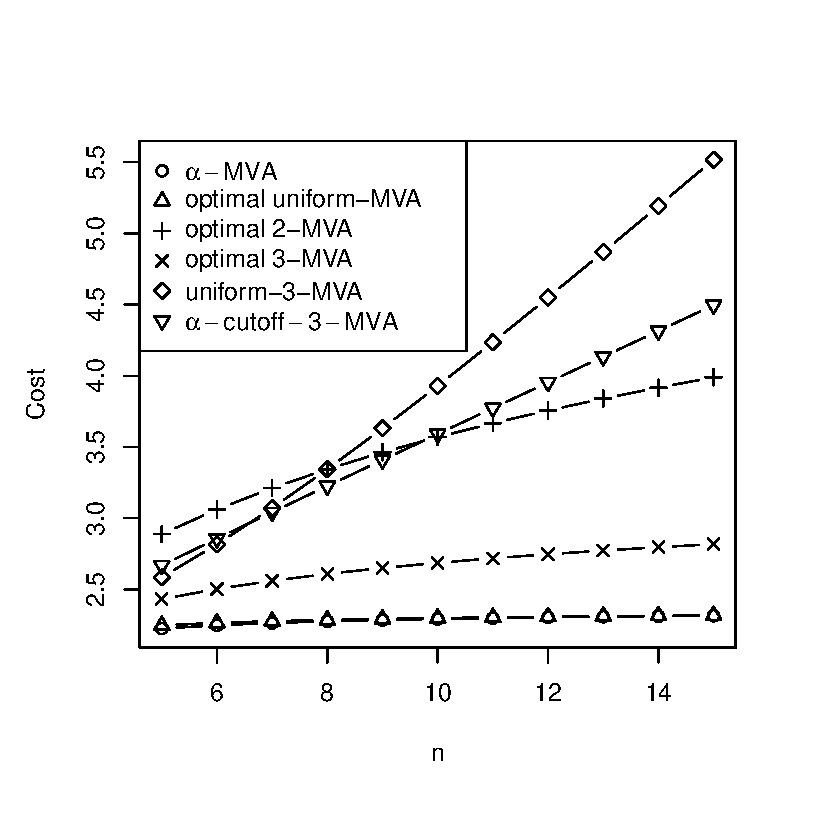
\includegraphics[trim=0 5mm 5mm 15mm, clip, width=.3\linewidth]{figures/analyze_cost_.5_5_15.eps}
%        \label{fig:cost_comparison_.5}
%    }
%    \subfigure[$\rho = 2$]{
%        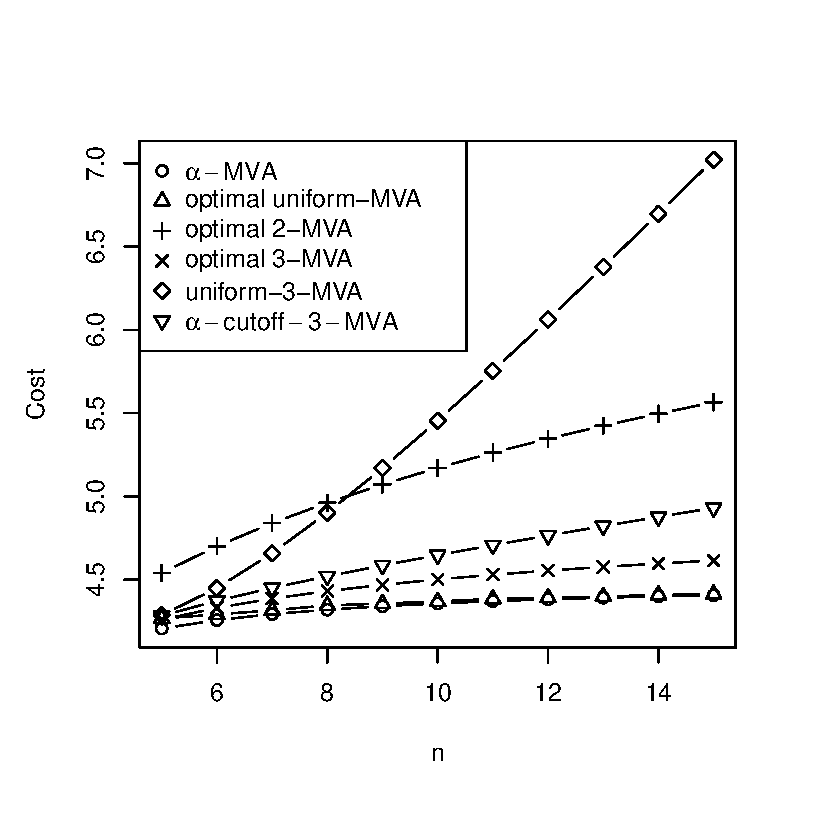
\includegraphics[trim=0 5mm 5mm 15mm, clip, width=.65\linewidth]{figures/analyze_cost_2_5_15.eps}
%        \label{fig:cost_comparison_2}
%    }
    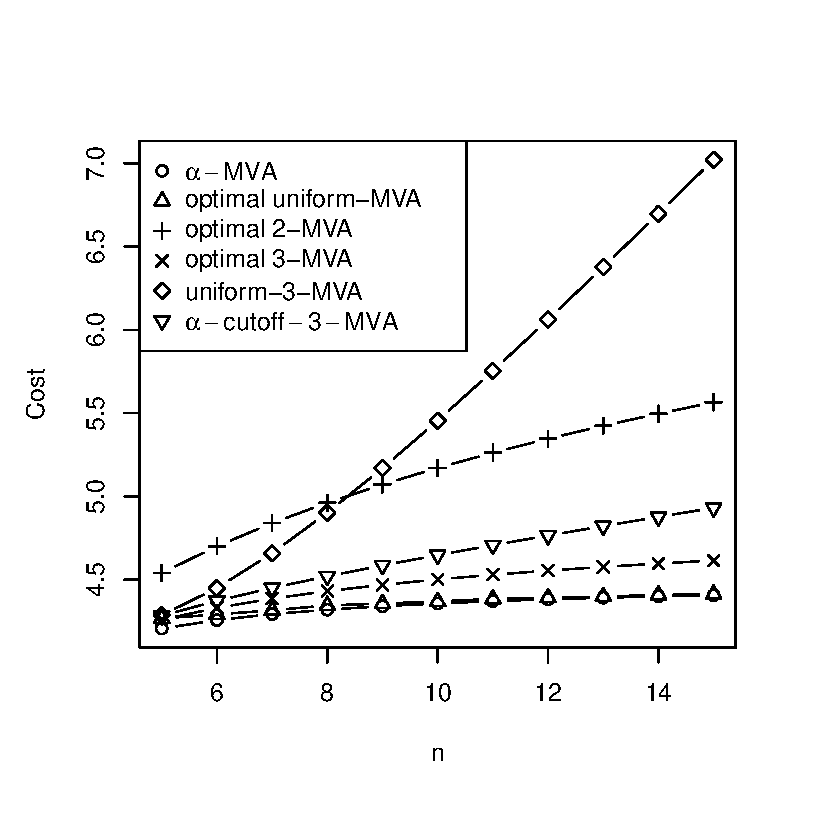
\includegraphics[trim=0 5mm 5mm 15mm, clip, width=.65\linewidth]{figures/analyze_cost_2_5_15.eps}
    \label{fig:cost_comparison_2}
    \caption{Comparing the costs of different MVAs over the number of bidders $n$. ($b = 2$, $c=1$)}
    \label{fig:cost_comparisons}
\end{figure}
\begin{itemize}
\item 
The optimal uniform-MVA's cost is very close to that of the optimal $\alpha$-MVA,
especially when $n$ is large. This makes sense because when $n$ grows
large, the optimal $\alpha$ approaches $1$, so the first few queries of
the optimal $\alpha$-MVA are at similar distances from each other.
%That is probably because
%    \begin{enumerate}
%        \item $\alpha$ approaching $1$ when $n$ grows large, which makes the
%        first $k$ thresholds $\alpha, \alpha^2, \alpha^3, \ldots, \alpha^k$
%        close to uniform thresholds $1-(1-\alpha), 1-2(1-\alpha), \ldots,
%        1-k(1-\alpha)$; 
%
%        \item the probability that the highest value falls out of first $k$
%        thresholds, $\alpha^{nk}$, becomes negligible for large $n$.
%    \end{enumerate}
\item The optimal $k$-MVA's cost decreases and approaches the optimal cost quickly
as $k$ grows.
% (check optimal $2$-MVA and $3$-MVA).
\item When $k$ is fixed to a small value, 
the uniform $k$-MVA  has significant higher cost than both the optimal
$k$-MVA and the $\alpha$-cutoff-$k$-MVA.
\item The $\alpha$-cutoff-$3$-MVA works well (close to optimal $3$-MVA).
%as shown in figure \ref{fig:cost_comparison_.5}. 
%but it is not
%as good as  the optimal $2$-MVA when $\rho$ is small and $n$ is large. 
%as shown in
%figure \ref{fig:cost_comparison_2}. Thus find the right thresholds is even more
%important than adding one more round in those cases.
\end{itemize}


\section{Optimal Mechanisms with Both Seller's and Bidder's Cost}
\label{sec:general}

In this section, we take out the constraints and prove that MVAs are optimal in
general. We will also try to find the specific MVA to achieve such optimality,
which turns out to be significantly more complex than previous
simplified case.

Let us first look at bidder's bid cost.  Sending emails, making phone
calls, enterring credit card nubmers, depositing money and clicking buttons are
all costly for bidders, though sometimes very tiny.  Bidders may not bid when
this cost is greater than their expected utility. Note that even if the
valuation is very high, the expected utility can be very small because of tense
competition, which is very common on the Internet as $n$, the number of
potential bidders, is very large.

%The first constraint we are going to remove is seller's cost only.  It is
%exciting to introduce bidder's bid cost since it occurs very often in real
%cases and it plays an important role.  Sending emails, making phone calls,
%enterring credit card nubmers, depositing money and clicking buttons are all
%costly for bidders, though sometimes very tiny.  Bidders may not bid when this
%cost is greater than their expected utility. Note that even if the valuation is
%very high, the expected utility can be very small because of tense competition,
%which is very common on the Internet as $n$, the number of potential bidders,
%is very large. 

This behaviour (bidders will not bid because of competitions) is very different
compared to that in previous model \cite{McAfee97:SequentialAuctions} of
sequential auctions. In that model, there is a time discount which
makes bidders eager to bid in early rounds with high reserve prices to avoid
waiting lost. 
%That makes a lot sense in some cases but sometimes it may not.
%For example, 
Suppose that the seller posts an auction with a very low reserve price in
the first round, most bidders with high valuation must be happy to bid
according to that time discount cost model. But in our model, a lot bidders
may be reluctant to bid because of competence, which can hurt seller's revenue.
%But this may not be true. For
%example, when I encounter such an auction online \footnote{For example, when I
%see a very good item in the Auction House of Diablo III with a very low current
%bidding}, I might be very reluctant to bid because there is a big probability
%that my bidding will be over taken by someone else's so it is just a waste of
%effort. Our cost model can describe this behaviour very well.

%Assume an extreme case where the broadcast cost is $0$, the bidder's bidding
%cost is $0.1$ and there are $n \rightarrow \infty$ many $[0, 1)$-uniform
%distributed bidders. In a Dutch auction (a Dutch auction has infinite many
%rounds of broadcasts so we have to set braodcast cost to $0$), only one bidder
%is expected to bid (no competition), thus every bidder with a valuation $v_i
%> 0.1$ should be benifitable to bid when the reserve price drops to a little
%bit below $v_i-0.1$ (recall that $n \rightarrow \infty$).  In a Vickrey
%auction, however, the competition is very tense. Only bidders with valuation
%greater than $t$ can accept such intense competition where $t$ satisfies
%$t^{n-1}t - 0.1 = 0$ (the expected utility for a bidder with valuation $t$ is
%$0$).  Thus $t = \sqrt[n]{0.1}$ which is arbitrary close to $1$ as $n$ grows to
%infinity.  Thus almost all bidders cannot bare this competition when $n$ is
%really large.
%
%So a mechanism (e.g. a Vickrey auction) with too much bidders' bid cost
%(competence) will have less participations and therefore may decreases seller's
%profit significantly.  To see this, look at previous extrame case again.  The
%revenue of Dutch auction will converge to $0.9$ (someone with valuation very
%close to $1$ will bid for price very close to $0.9$) when $n$ becomes infinity.
%The revenue of a Vickrey auction, however, is only $\int_t^1 x \, (n-1) \,n\,(
%1-x) \,{x}^{n-2} dx$ which converges to about $0.67$ when $n$ grows to
%infinity.  

The bidder's bid cost will also make revenue equivalence theorem no longer
applicable.  That is not strange as the revenue equivalence theorem assumes
that the utility of a bidder winning the item is equal to the valuation minus
the payment. This assumption is no longer true as now the utility is also
influenced by the cost charged to this bidder. And even if the bidder doesn't
win, the cost still exists so we can't simply revise the valuation.

Therefore, the first issue we are going to solve is to make a very similar
theorem applicable to our model again. 

\subsection{Spending Equivalence Theorem and Revenue Optimization Strategy}

\begin{theorem}\label{theorem:equivalence}

The expected overall spendings from bidders (including their bid costs and
payments to the seller) is completely determined by the expected utility of
lowest type bidders and allocation probability function
$$p: (v_1, v_2, \ldots, v_n) \rightarrow (p_1, p_2, \ldots, p_n)$$ 
where $p_i$ is the probability that bidder $i$ will get the item.

\end{theorem}

\begin{proof}
To prove it, let us construct another mechanism
$M'$ without bid cost from our mechanism $M$ with bid cost so $M'$ fits
into the original revenue equivalence theorem's model. Suppose there is a
virtual seller in $M'$, who collects valuations from all bidders at no cost (a
direct revelation mechanism). Then this virtual seller will make $n$ virtual
bidders delegating bidders to communicate with the true seller in our mechanism
$M$.  When our mechanism ends by allocating the item to virtual bidder $i$, the
virtual seller also allocate the item to the real bidder $i$. The payment from
each bidder $i$ to this virtual seller will be equal to the payment that
virtual bidder $i$ pays to our real seller plus all the bid costs charged
to virtual bidder $i$.
$M'$ will satisfy revenue equivalence theorem and
%Thus, from the real bidders' aspects, this mechanism
%$M'$ is just a direct revelation mechanism which will satisfy revenue
%equivalence theorem. 
the payment from real bidder
$i$ to the virtual seller has two parts, one payed to the real
seller, another consumed by bid costs, which sum up to total spending.
\end{proof}

Thanks to theorem \ref{theorem:equivalence}, our profit maximization problem
is now greatly simplified: 

\begin{corollary}
To maximize profit for a given allocation rule $p: (v_1, v_2, \ldots, v_n)
\rightarrow (p_1, p_2, \ldots, p_n)$, we only need find the minimum total cost
(including both seller's cost and bidders' cost).
\end{corollary}

\begin{proof}
The total spending, substracts cost charged to bidders, will be the revenue
that the seller receives.  This revenue, substracts cost charged to the seller,
will be profit. Thus profit is total spending minus total cost. As total
spending is fixed by allocation rule, we only need to find the minimum cost to
maximze profit.
\end{proof}

The highlight here is that we will not have to differentiate cost charged to
bidders and cost charged to sellers if we just want to maximize seller's profit.
The difference of them may make revenue different, but as long as their sum
does not change, the profit will not change. This not only helps us simplify our
analysis, but also helps us simplify the optimal mechanism: 

%\begin{figure*}
%\centering
%  \subfigure[Best query length $x$ over $h$ with fixed $l$]{
%    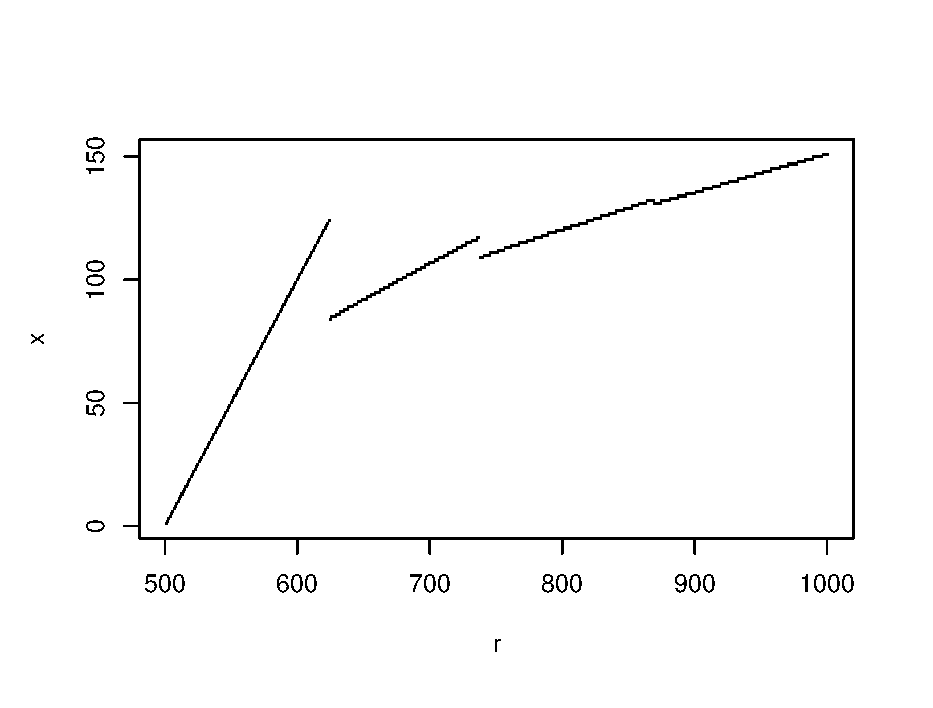
\includegraphics[trim=0mm 5mm 5mm 15mm, clip, width=.4\linewidth]{figures/1000-500-2-1-10}
%    \label{fig:x-h}
%  }
%  \subfigure[Normalized best query length $x$ over low value $l$]{
%    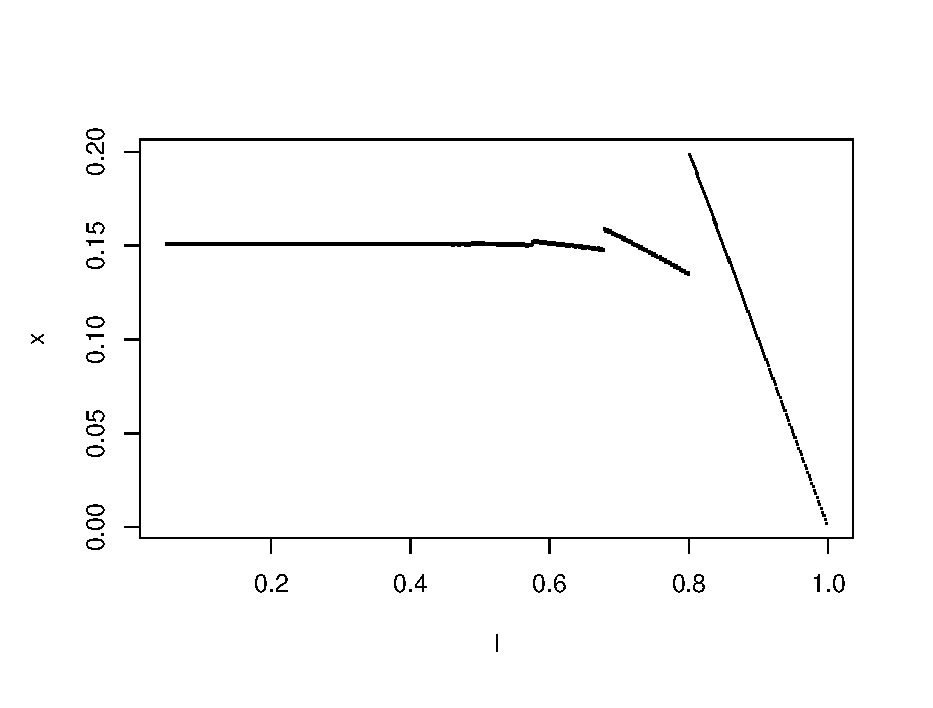
\includegraphics[trim=0mm 5mm 5mm 15mm, clip, width=.4\linewidth]{figures/10000-500-2-1-10}
%    \label{fig:x-l}
%  }
%  \caption{In the first subfigure, we plot the best query length $x = \hat x / D$ over $h = \hat h / D$ (the highest
%      undiscovered value) with discretized low value $\hat l = 500$,
%      broadcast bid cost ratio $\rho = 2$,
%      number of bidders $n = 10$ and maximum discretized valuation
%      $D = 1000$. In the second subfigure, we normalize $x$ to be $x = \hat x / \hat h$ and
%      $l$ to be $l = \hat l / \hat h$, as if $h$ is always $1$.}
%\end{figure*}

\begin{figure}
    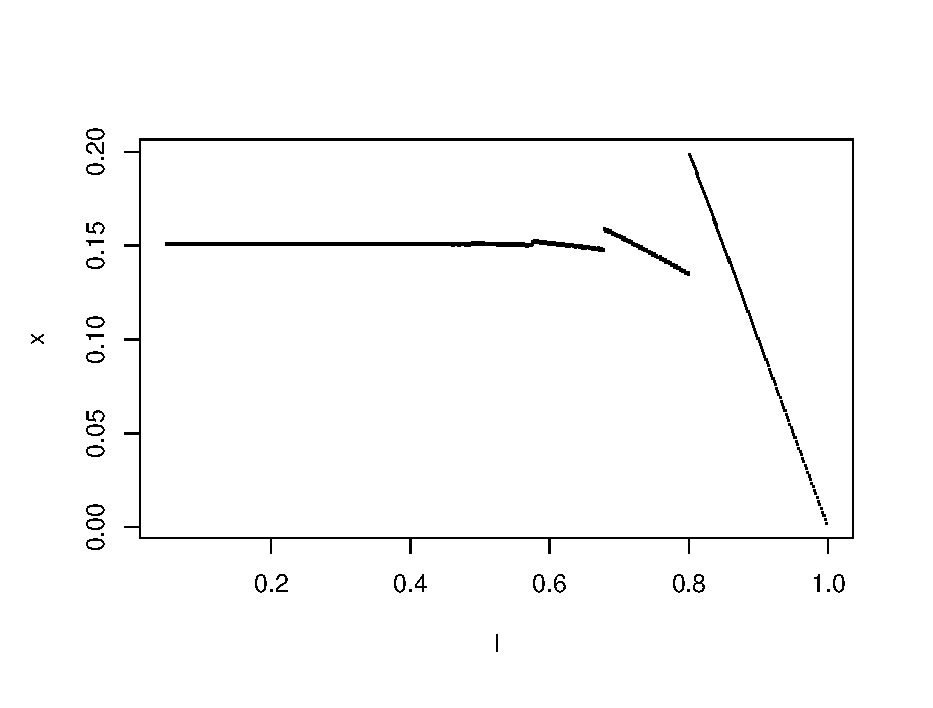
\includegraphics[trim=0mm 5mm 5mm 15mm, clip, width=\linewidth]{figures/10000-500-2-1-10}
    \caption{Best first-query-length $x$ over low value $l$. In the experiment, 
    we set $\rho=2$ and discretize $[0,1)$ into $1000$ grids.}
    \label{fig:x-l}
\end{figure}

\begin{proposition}
In original MVA, to make a set of thresholds $a_i$ works (the
equilibrium holds), we may have to make $r_i$ negative. That says, we need to
compensate bidders if only one bids at reserve price $r_i$ rather than charge
him something, in order to maintain bidders incentive to bid in spite of
bid cost. That's not intuitive and sellers/bidders may
not be able to easily understand it. A better way to achieve $a_i$ might be
compensating the bidder with the bid cost immediately after the bidding.
Equivalently, the seller buys the bid cost for bidders and make it as a
part of seller's bid cost. This won't change his profit but this will make
everything looks more intuitive ($r_i$ is non-negative again).
\end{proposition}

Since profit is total spending minus overall cost where total spending is
decided by allocation rule which is studied in Myerson's work, our optimizing
problem is greately related to Myerson's if we were able to minimize the
overall cost. However, the optimal allocation rule here is not as simple as the
one that is discovered by Myerson \cite{Myerson:1981}: allocate the item to the
bidder with highest positive virtural value.  Theorem \ref{theorem:equivalence}
tells us that this rule will maximize the total spending.  But we must
substract the cost from the spending to get the profit.  Therefore, there might
be another weird allocation rule that has less total spending but even much
less minimum cost.

%It is not hard to find one example of this. We know that for bidders
%with uniform valuation over $[0, 1)$, the spending maximizing allocation rule
%is allocate the item to the bidder with highest valuation that is greater than $1/2$.
%However, if the broadcast cost is too large, for example $1$ (which is equal to the
%highest possible valuation), the cost to find out whether there is any bidder with valuation
%greater than $1/2$ is at least $1$. Thus if we use this allocation rule, the
%final profit would be negative since the total spending must be less than the
%minimum cost. However, the allocation rule that never allocate the item will have
%$0$ cost and $0$ spending, which achieves $0$ profit, better than previous allocation
%rule.

Thus, the profit optimal mechianism will depend on how minimum cost is defined given an allocation rule. 

%We previously defined how cost is charged and proved that a specific mechanism (MVA)
%has minimum cost when allocation rule is allocate efficiently. But unfortunately,
%that is not enough to give us a well defined minimum cost for any allocation rule.
%For example, one allocation rule might be always allocate the item to each bidder
%with the same probability $1/n$, i.e. $p(v_1, v_2, \ldots) = (1/n, 1/n, \ldots)$.
%One might think that the minimum cost for this is $0$ since we do not have to know
%anyone's valuation. But that cost is not realistic: how can the mechanism ever allocate the
%item to someone that it has never communicated with? Thus the minimum cost seems
%to be at least $b$, the cost for one round of broadcast, if we ever allocate the item
%to some bidder. In order to make a realistic constraint and get a well defined minimum
%cost for any allocation rule, we define

\begin{definition}\label{def:allocation_cost}
A mechanism with allocation rule $$p: (v_1, v_2, \ldots, v_n) \rightarrow
(p_1, p_2, \ldots, p_n)$$ does not allocate blindly if it satisfies: if $p_i >
0$ for some valuation profile $(v_1, v_2, \ldots, v_n)$, there must be a
broadcast query that the $i$-th bidder ($v_i$) reply to the seller
under that profile setting.
\end{definition}

The no-blind-allocation property defined above will ensure the optimality
(minimum cost) of the following mechanisms.

\begin{definition}

Mechanisms satisfy relaxed efficiency constraint with low value $l$
if they always allocate the item to the bidder with highest valuation that's
at least $l$ (no allocation if everyone is below $l$).
%
%    \begin{enumerate}
%
%    \item They only allocate the item to bidders whose valuation are at least
%    $l$ (the low value is $l$)
%
%    \item If they will allocate the item, they will always allocate the item to
%    the bidder with highest valuation.
%
%    \end{enumerate}
%
When we say a mechanism has a low value $l$, we imply that it
satisfies relatex efficiency constraint with low value $l$.

\end{definition}

%With this definition, we have

\begin{theorem}
In regular cases (the virtual valuation is monotone strictly increasing~\cite{}),
mechanisms satisfying relaxed efficiency constraint with some low value $l$ are
optimal among all mechanisms that won't allocate blindly.

%The optimal mechanism should always allocate the item to the bidder with
%highest virtual valuation $v_i - \frac{1-F(v_i)}{f(v_i)}$ if it decides to
%allocate the item. In regular cases when the virtual valuation is monotone
%strictly increasing, the optimal mechanism should always allocate the item to
%the bidder with highest valuation if it decides to allocate the item.
\end{theorem}

\begin{proof}
Suppose that there's an arbitrary optimal mechanism. We can describe it by a
query strategy $S(f, m, V, \mathcal Q)$ (see definition \ref{def:query}) and an
allocation function based on $V$, the set of reported values set, since we can
only allocate item to reported bidders. We then construct another mechanism
with query strategy $S'(f, m, V', \mathcal Q')$ where $\mathcal Q'$ are decsending
and 
\begin{align*}
|S'(f, m, \emptyset, \{Q'_1, \ldots, Q'_{i-1}\})| %= |Q'_i| = |Q_i|\\
  = |S(f, m, \emptyset, \{Q_1, \ldots, Q_{i-1}\})|
\end{align*}
That says, if there's no reported bidders yet, we will always ask the
descending query which has the same length as the query of $S$. And we pretend
that we asked the same query as $S$ so we can continue to ask $S$ what's the
next query length. Once we get reply in $S'$, we terminate the mechanism
immediately and allocate the item to the replied bidder with highest valuation
with probability 1.  Note that we may have $|Q'_i| = |Q_i| = 0$ which means
both mechanisms terminate after $i$ queries without any reply and allocation.
It's clear that our new mechanism won't cause more cost than original
mechanism.  And our new mechanism's allocation rule will get at least as high
total spending as original mechanism because it makes allocation probability of
high value bidders as much as possible. Therefore our new mechanism, which
satisfies relaxed efficiency constraint with some low value $l$, is also
optimal.
%Firstly, note that (at least one) optimal allocation rule $p$ will have at most
%one possible winner, i.e. there can't be $p_i, p_j > 0$ if $i \neq j$. If not,
%without loss of generality let's suppose $v_i \geq v_j$ and $p_i, p_j > 0$. We
%can shift $j$'s probability to $i$, making $p_i' = p_i + p_j$ and $p_j' = 0$.
%Since it can't allocate blindly, this won't increase the cost and actually it
%can potentially lower the cost because we don't need bidder $j$ to reply.  The
%total spending is also non-decreasing by this change in regular cases thus the
%profit is non-decreasing. Keep on doing this change will eventually give us an
%optimal allocation rule with only one possible winner.
%
%Secondly define active region $A$ as
%\begin{align*}
%  A = \{ v_i ~|~ \exists (v_1, \ldots, v_i, \ldots, v_n), p_i > 0 \}
%\end{align*}
%
\end{proof}

For simplicity, we will always assume regularily and will not mention virtual
valuation below.  It's easy to extend our result to general cases by mapping
all values to virtual values and ask broadcast queries according to virtual
values.

\subsection{MVAs' Optimality in General}

We have already narrowed down optimal mechanism to
relaxed efficient mechanisms and by theorem \ref{theorem:equivalence},
it is straightforward to see

\begin{corollary}

For mechanisms with a fixed low value $l$, the maximum profit is
achieved when the mechanism minizes the cost.

\end{corollary}

Our next question is naturally: what is the cost minimized mechanism
given a low value $l$. 
A similar lemma can be proved using almost identical technique to lemma \ref{lemma:uniform}.
Thus for space limit, we will not elaborate it again. 

\begin{lemma}\label{lemma:lowest_type}
Suppose that there are two cases $n, F_1, f_1, l_1$ and $n, F_2, f_2, l_2$
where $n$ is the number of values for both cases, $F_i, f_i$ are CDF and PDF
of the $n$ i.i.d. values in case $i$, $l_i$ is the low value for case $i$.
If $F_1(l_1) = F_2(l_2)$, then these two cases have the same minimum cost
to find the maximum value above the low value $l_i$.
\end{lemma}

Finally, we conclude

\begin{theorem}

MVAs have the minimum cost among all mechanisms with a low value $l$. Thus
they are optimal.

\end{theorem}

\begin{proof}
A special case of this theorem when $l = 0$ is theorem \ref{theorem:MVA_eq}.
We proved that special case by introducing lemma \ref{lemma:uniform} and
\ref{lemma:descending}. To prove the general cases with arbitrary $l$, we just
need to revise lemma \ref{lemma:uniform} a little to lemma
\ref{lemma:lowest_type}. All other part of the proof remains similar. For space
limit, the detailed proof is omitted.
\end{proof}

Then the only parameters we are going to determine for the
specific optimal MVA are 1) the low value $l$; 2) the descending query
thresholds $a_1, a_2, a_3, \ldots$.
When we later investigate such parameters that minimizes the cost, we will
also assume uniform distribution $F(x) = x$ in default because distribution will not
change this minimum cost and we can always adapt an optimal MVA for uniform distribution
to an optimal MVA for any distribution easily.

%\subsection{Experiments to Discover Optimal MVA with a Given Low Value}
%
%To discover the specific MVA that is optimal, we first try to identify the
%optimal thresholds $a_i$ given a low value $l$  (recall that in $i$-th round,
%MVA will ask all bidders whose valuation is within $[a_i, a_{i-1})$ to bid).
%If we can write the minimum cost $C^*$ as a function of $n, \rho, l$ (recall
%that $\rho = b/c$ is the ratio between broadcast and bid cost), we may then
%determine the optimal $l$ by that.
%
%%In the special case that we studied in previous section where $l = 0$
%%(efficiency is enforced), the optimal thresholds can be easily described as a
%%single parameter $\alpha$. This strategy will not work when $l > 0$ (we assume uniform
%%distribution in default). Obviously that $a_i \geq l$,
%%thus we cannot let $a_i = \alpha a_{i-1}$ since $\lim_{i \rightarrow \infty} a_i
%%= 0 < l$.  Additionally, if we revise the equation by letting $a_i-l = \alpha
%%(a_{i-1}-l)$, we will get a positive possibility $F(l)$ that we would ask
%%infinite many broadcast queries, which is even worse.
%
%As it is not immediately clear what optimal thresholds should be like, we
%present a simple algorithm to calculate such thresholds numerically. We firstly
%discretize the continuous valuation $[0, 1)$ to $D$ discrete values $\{0, 1, \ldots,
%D-1\}$. That means, the original valuation $v$ will be transformed to integer
%value $\hat v = \lfloor v D \rfloor$. Then we use dynamic programming to
%inductively calculate $\hat x_{\hat h}$, the length of next optimal descending
%query $[\hat h-\hat x_{\hat h}, \hat h)$ to ask, conditional on that we have
%already queried $[\hat h, D)$ and no one replies.
%
%\begin{algorithm}
%    \caption{Calculate discretized best query lengths}\label{algo:discrete}
%    \begin{algorithmic}[1]
%        \Require{$\hat l$ is the discretized low value, $\rho$ is the ratio between broadcast and bid cost,
%        $n$ is the number of bidders, $D$ is the maximum discretized valuation}
%        
%        \Function{BestQueryLengths}{$\hat l$, $\rho$, $n$, $D$}
%            \State $\hat x_{\hat l} \gets 0$
%            \State $C_{\hat l} \gets 0$
%            \For{$\hat h={\hat l}+1 \mbox{ to } D$}
%                \State $\hat x_{\hat h} \gets \displaystyle
%                  \operatorname*{arg\,min}_{1 \leq \hat x \leq \hat h-l} \rho + n
%                  \frac{\hat x}{\hat h} + (\frac{\hat h-x}{\hat h})^n C_{\hat h-\hat x}$
%                \State $C_{\hat h} \gets \rho + n \frac{\hat x_{\hat h}}{\hat h} +
%                  (\frac{\hat h-\hat x_{\hat h}}{\hat h})^n C_{\hat h-\hat x_{\hat h}}$
%            \EndFor
%            \State \Return $\hat x$
%        \EndFunction
%    \end{algorithmic}
%\end{algorithm}

\begin{figure*}
\centering
    \subfigure[$n = 10, b = 0.2, c = 0.1$]{
      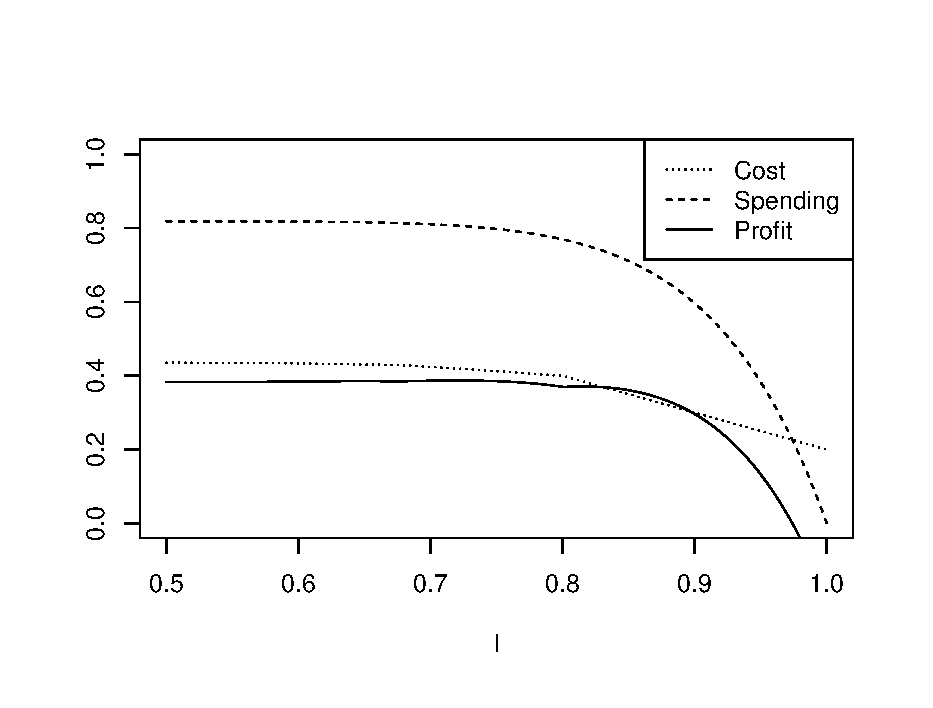
\includegraphics[trim=0mm 5mm 5mm 15mm, clip, width=.32\linewidth]{figures/10-0.200000-0.100000.eps}
      \label{fig:CSP-l-2-1}
    } 
    \subfigure[$n = 10, b = 0.5, c = 0.1$]{
      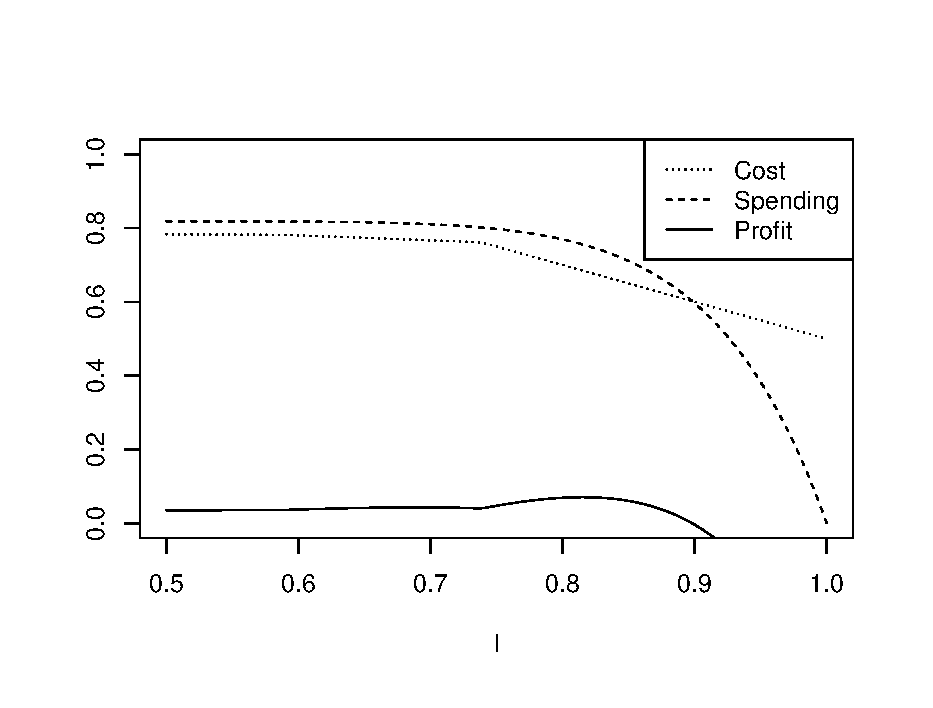
\includegraphics[trim=0mm 5mm 5mm 15mm, clip, width=.32\linewidth]{figures/10-0.500000-0.100000.eps}
      \label{fig:CSP-l-5-1}
    }
    \subfigure[Suboptimality, $n = 10, b = 0.2, c = 0.1$]{
      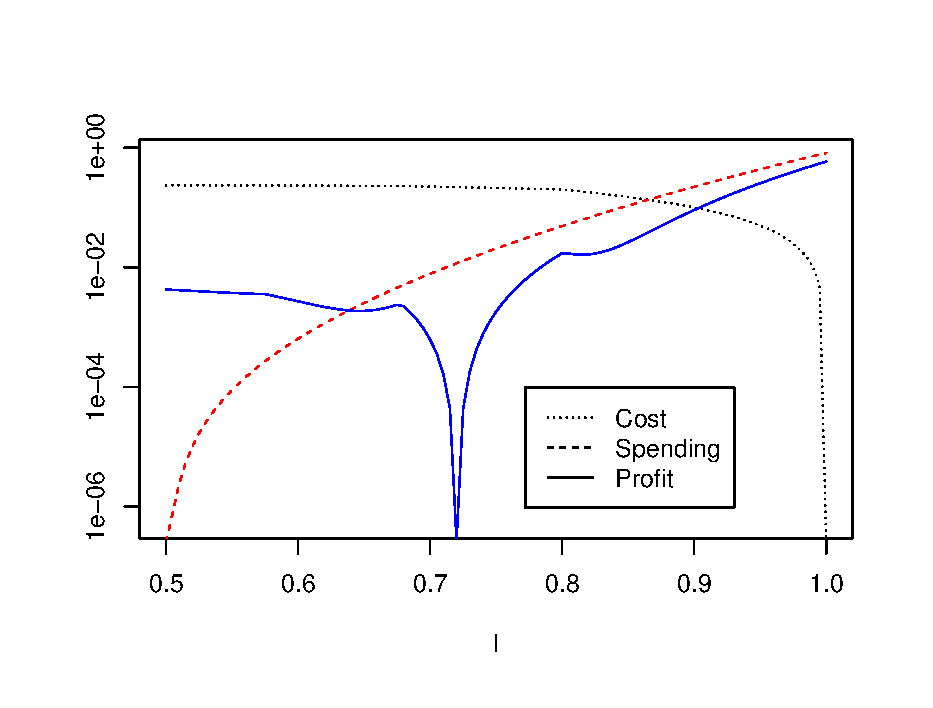
\includegraphics[trim=0mm 5mm 5mm 15mm, clip, width=.32\linewidth]{figures/suboptimality.eps}
      \label{fig:suboptimality}
    }
    \caption{Optimal MVA's cost, spending, profit over $l$, $n$ i.i.d. uniform distributed bidders,
      broadcast $b$ and bid cost $c$}
\end{figure*}

%Algorithm \ref{algo:discrete} runs in time $O(D^2)$. Having $\hat x$, we can
%then infer the best strategy $x$ for original continuous problem by converting
%$\hat h, \hat x$ back to $h, x$ and using them to interpolate continuous
%strategy.  The larger $D$ is the more accurate it will be. But it will also
%require more running time.  Running this for case $l = .5, \rho = 2, n = 10, D
%= 1000$ we get $x$ showed in figure \ref{fig:x-h}. It seems that $x$ is a
%piecewise linear function over $h$.  For those $h$ which is close to
%$l$, obviously that the optimal strategy should be $x = h - l$,
%which means using only one query to explore all potential bidders. But it is
%unclear why $x$ is linear when the best strategy is using multiple queries to
%explore the valuation range.
%
%Another way to plot the graph is to normalize $x$ and $l$ so that $h$ becomes
%$1$ since our model is $v_i \in [0, 1)$. It is showed in figure \ref{fig:x-l}.
%This again looks like a piecewise linear function.  A more interesting
%observation is that the left-most piece is quite a long straight line $x =
%1-\alpha$. Thus it seems that $x = 1-\alpha$ is optimal for quite a lot $l$ which is not
%far from $0$. Here the $\alpha$ is the the optimal $\alpha$ of $\alpha$-MVA if
%we set $l = 0$.

\subsection{Analysis of Optimal MVA with a Positive Low Value}\label{sec:general_analysis}

Before an analytical treatment, we first conduct an experiment to compute the
optimal MVA approximately for getting some insights. In that experiment, we
discretize the value into fine grids and then use dynamic programming to
compute the optimal first-query-length over different $l$ (this is sufficient to derive the whole
optimal MVA because a failed query is equivalent to increase the $l$ after
renormalizing). The result is plotted in Figure~\ref{fig:x-l}
and it seems to be much more complicated than $\alpha$-MVA but there might
still be hope to get a nice analytical result: it seems like a piecewise linear
function. Specifically, we cannot use a single $\alpha$ to describe such
optimal MVA, but perhaps we can use a sequence of $\alpha$ to describe it. Now
let us take an analytical treatment.

%Figure \ref{fig:x-h} shows that the optimal MVA with a low value $l > 0$ is
%much more complicated but there might still be hope to get a nice analytical
%result: piecewise linear function. That is, we cannot use a single $\alpha$ to
%describe such optimal MVA, but perhaps we can use a sequence of $\alpha$ to
%describe it. Now let us take an analytical treatment.

The first key to analyze the optimal MVA with $l > 0$ is to utilize
the fact that there is a maximal number of rounds to exploit the whole
reportable valuation range $[l, 1)$. Let us call that
number $k$.\footnote{We have argued this before: if such $k$ does not exist, or equivalently
the maximum number of rounds is unbounded, the cost will be infinite as the possibility that no
values lie in $[l, 1)$ is positive.}

For convenience, define $\boldsymbol a = (a_0, a_1, a_2, \ldots, a_k)$, the vector of
thresholds in such optimal MVA. We make $a_0 = 1, a_k = l$ so in $i$-th
round the query would be $[a_i, a_{i-1})$. Now define cost $C(\boldsymbol a, k, \rho,
n)$ to be the expected cost for MVA defined by $k, \boldsymbol a$ when there are $n$
i.i.d.  $[0, 1)$-uniform bidders (note that $l, h$ are implicitly defined by
$a_k, a_0$). If we can get a neat form of $C$, we can use $\frac{\partial
C}{\partial a_i} = 0 $ to characterize optimal MVA, as we did in 
\ref{sec:alpha-MVA}.\footnote{It is easy to see that boundary cases $a_i = a_{i-1},
a_{i+1}$ are not optimal too.}

Thus the second key is to represent this $C$. Rather than
considering one round after another recursively as we did before, we now consider all
rounds together. Let $CR_i$ denote the cost that occur in round $i$ (the broadcast
of that round and the bid cost charged in that round) and $v^* = \max_i v_i$. Then expected cost
would be sum of expected cost of each round:
\begin{align}
C(\boldsymbol a, k, \rho, n) &= \sum_{i=1}^k E[ CR_i ] \nonumber \\
  &= \sum_{i=1}^{k} \Pr\big( v^* < a_{i-1} \big) E[CR_i ~|~ v^* < a_{i-1}] \nonumber \\
  &= \sum_{i=1}^{k} \frac{a_{i-1}^n}{a_0^n} \left( \rho + \frac{a_{i-1}-a_{i}}{a_{i-1}} n \right)
  \label{eq:C_general_simplified}
\end{align}

Taking derivative we get
\begin{align}
 \frac{\partial C}{\partial a_i} = \frac{
	n(n+\rho)a_i^{n-1}-n(n-1)a_{i+1}a_i^{n-2}-n a_{i-1}^{n-1} }{a_0^n}
	\label{eq:diff_C_general}
\end{align}

Unfortunately, equation
\ref{eq:diff_C_general} is not neat enough to get a piecewise linear query length.
Recall that in previous subsection, the experiment seems to show that query length $x$ is
piecewise linear over $l$, which means $a_1 = a_2+x = l+x$ must also be
piecewise linear over $a_2 = l$.  One counter example is the simple case $k =
2, n = 3$. We have: $a_1 =
(\sqrt{{a_0}^{2}\,\rho+{a_2}^{2}+3\,{a_0}^{2}}+a_2)/(\rho+3)$.  Anyway, by
definition we have $a_1 \geq a_2$. And the former equation indeed looks very
linear when $a_1 \geq a_2$.

Though we failed characterizing the optimal MVA using piecewise linear
functions, equation \ref{eq:C_general_simplified} gives us a better way to
calculate thresholds $a_i$. We use an R package called BB \cite{Varadhan2009:BB} to
solve these non-linear equation systems. Before throw those equations to that
package, we have to first decide $k$ and an initial guess of $\boldsymbol a$.

We found a lemma that's very useful for deciding $k$:

\begin{lemma}\label{lemma:thresholds}
Two vectors of optimal thresholds $\boldsymbol a = (a_0, \ldots, a_k)$ and
$\boldsymbol a' = (a'_0, \ldots, a'_m)$ can't have $p_2 \leq q_2 < q_1 < p_1$
where $p_2, p_1$ and $q_2, q_1$ are two consecutive thresholds $a_i, a_{i-1},
a'_j, a'_{j-1}$.
\end{lemma}

\begin{proof}
Denote $C(l)$ to be the optimal cost for finding the maximum value above low
value $l$ (suppose $h, n, \rho$ and everything else are constants now). Note
that thresholds $a_0, \ldots, a_i$ must be optimal thresholds for $l = a_i$,
otherwise $a_0, \ldots, a_k$ can't be optimal for $l = a_k$.  Similarly,
$a'_0, \ldots, a'_j$ must be optimal thresholds for $l = a'_j$.  Then 
%from optimality of $a_0, \ldots, a_i$ and $b_0, \ldots, b_j$ we have:
\begin{align*}
%  C(b_{j-1}) + b_{j-1}^n [\rho+n(b_{j-1}-b_j)] \leq C(a_{i-1}) + a_{i-1}^n [\rho + n(a_{i-1}-b_j)]\\
%  C(a_{i-1}) + a_{i-1}^n [\rho+n(a_{i-1}-a_i)] \leq C(b_{j-1}) + b_{j-1}^n [\rho + n(b_{j-1}-a_i)]
  C(q_1) + q_1^n [\rho+n(q_1-q_2)] \leq C(p_1) + p_1^n [\rho + n(p_1-q_2)]\\
  C(p_1) + p_1^n [\rho+n(p_1-p_2)] \leq C(q_1) + q_1^n [\rho + n(q_1-p_2)]
\end{align*}
Adding these two inequations together and do some cancellations we get
$p_1^n \leq q_1^n$, which contradicts $q_1 < p_1$.
\end{proof}

From that we derive an upper bound for $k$. Intuitively, it says we will need
less rounds if we have less reportable range (a greater $l$).

\begin{lemma}\label{lemma:k_upper}
$k_\alpha = \left\lceil \log_{\alpha} \left(1/l\right) \right\rceil$ is an
upper bound for the optimal $k$. Here $\alpha$ is the optimal $\alpha$ for
$\alpha$-MVA when $l = 0$. 
\end{lemma}

\begin{proof}
We will prove by contradiction. Assume $k > k_\alpha$ for optimal thresholds
$(a^*_0, a^*_1, a^*_2, \ldots, a^*_k)$ where $a^*_0 = 1, a^*_k = l$ as defined.  Points
$a_0 = \alpha^0, a_1 = \alpha^1, \ldots, a_{k_\alpha} = \alpha^{k_\alpha}$
split interval $[l, 1)$ into $k_\alpha$ subintervals $[a_i, a_{i-1})$, which
together contain $k$ thresholds $a^*_1, \ldots, a^*_k$. Since $k > k_\alpha$, at
least one subinterval $[a_i, a_{i-1})$ contain two thresholds $a^*_j, a^*_{j-1}$.
Equivalently, there exists $a_i \leq a^*_j < a^*_{j-1} < a_{i-1}$.  This
contradicts with Lemma~\ref{lemma:thresholds}.
\end{proof}

\begin{figure}
\centering
    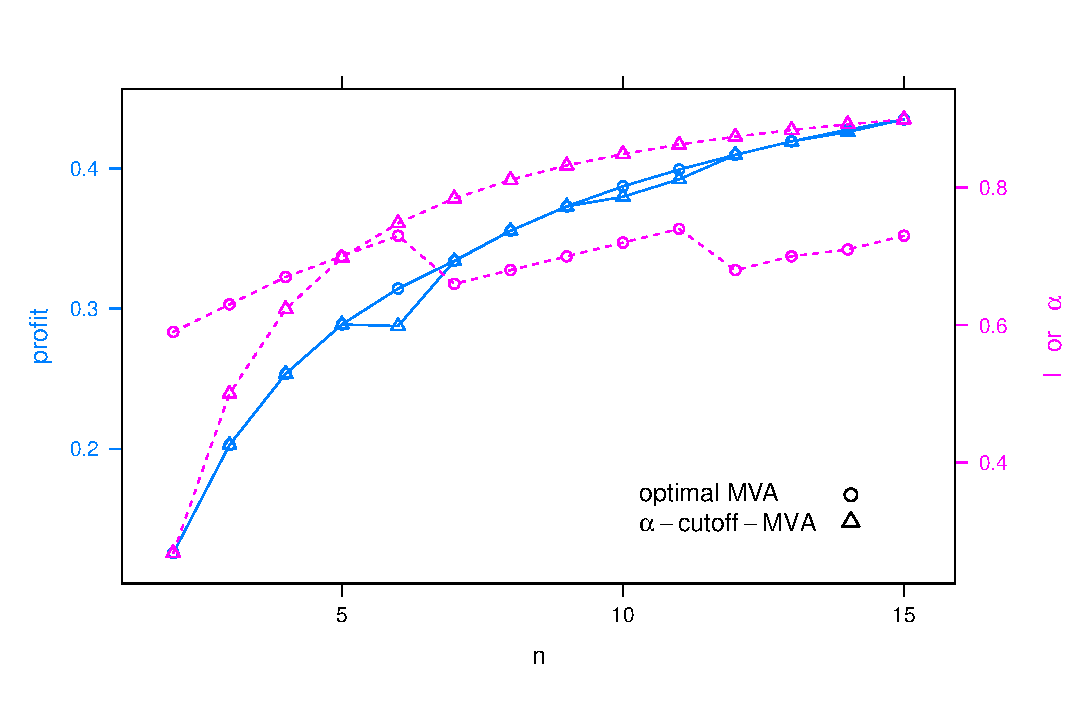
\includegraphics[width=\linewidth]{figures/cutoff_.2_.1_15.eps}
    \caption{The profit of optimal MVA and $\alpha$-cutoff-MVA are plotted in
    solid line.  The low value $l$ is chosen to maximze optimal MVA's profit.
    We also plot $l$ and $\alpha$ in dashed lines to see how they affect the
    relative profit difference.  Note that $\alpha$ does not depend on
    $l$.}\label{fig:cutoff}
\end{figure}

\begin{figure*}
\centering
  \subfigure[profit]{
    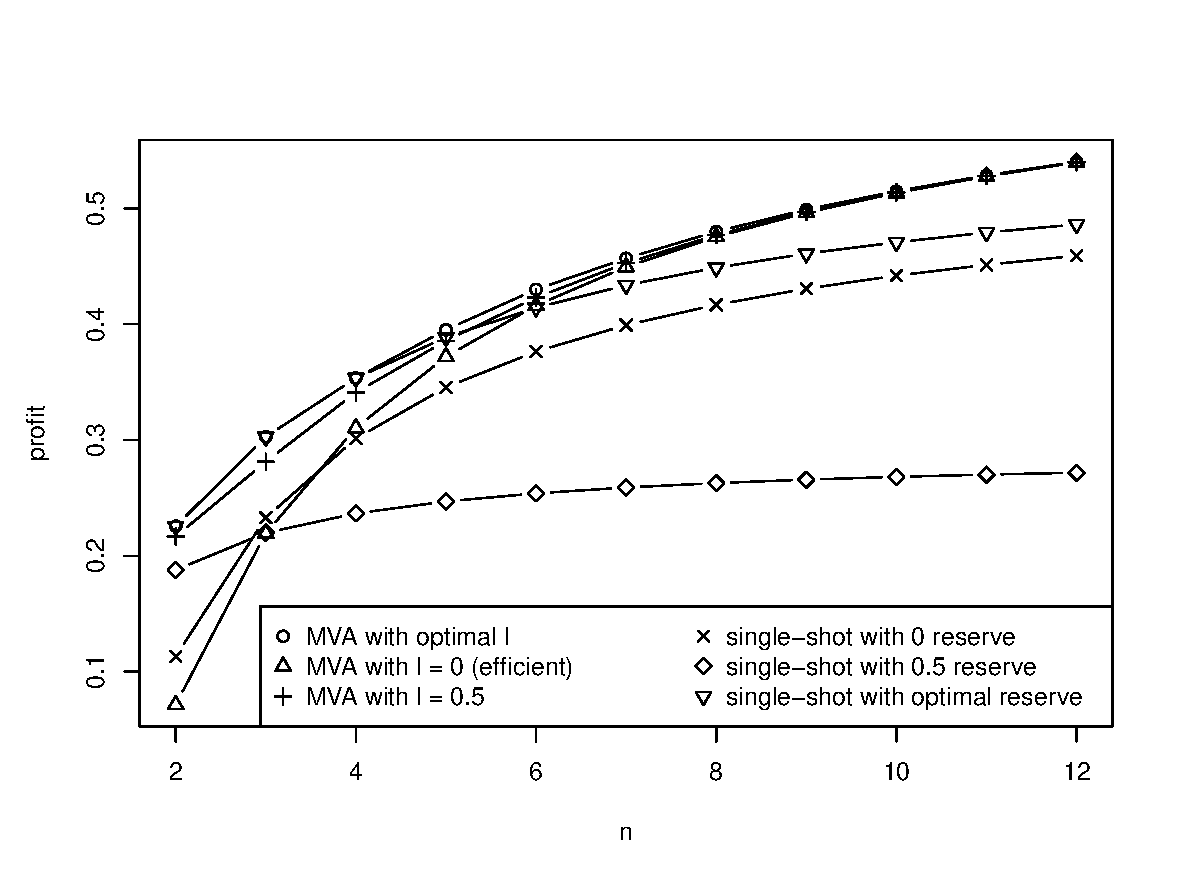
\includegraphics[trim=0mm 5mm 5mm 15mm, clip, height=.3\linewidth, width=.4\linewidth]{figures/profit_.1.eps}
    \label{fig:general_profit}
  }
  \subfigure[low value]{
    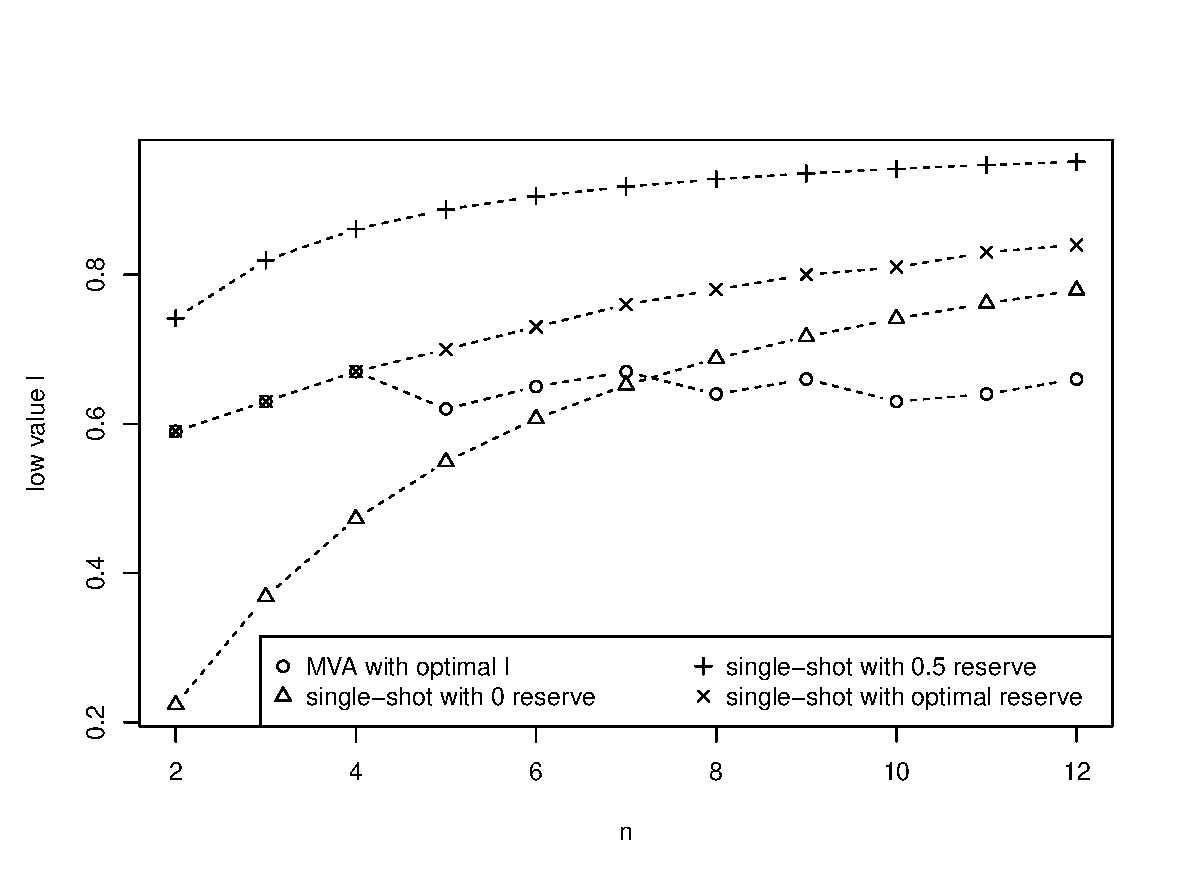
\includegraphics[trim=0mm 5mm 5mm 15mm, clip, height=.3\linewidth, width=.4\linewidth]{figures/l_.1.eps}
    \label{fig:general_l}
  }
  \caption{Compare profit and corresponding low value $l$ over $n$. The
  broadcast cost $b = 0.1$. Bidding cost for seller and buyer are $\beta_1 =
  \beta_2 = 0.05$ (thus $c = \beta_1+\beta_2 = 0.1$)}\label{fig:general}
\end{figure*}

Having this upper bound, we can eigther bruteforcely search all $k$ between $1$
and $k_\alpha$, or use ternary search [cite wiki?] to get optimal $k$ in
$O(\log k_\alpha)$ time if we can prove it is unimodal.\footnote{We did not
prove that it is unimodal but experiments seems to support this property.}
But in light of the proof above, we actually could have something much better:

\begin{theorem}\label{theorem:k_bounds}
$\left\lceil \log_{\alpha} \left(1/l\right) \right\rceil$ and 
$\left\lfloor \log_{\alpha} \left(1/l\right) \right\rfloor$ are upper
and lower bounds for the optimal $k$. 
\end{theorem}

\begin{proof}
We have proved the upper bound in Lemma~\ref{lemma:k_upper}. Similarly, if the lower bound
does not hold, we have $a^*_j = p_2 \leq \alpha^i = q_2 < \alpha^{i-1} =
q_1 < a^*_{j-1} = p_1$ which violates Lemma~\ref{lemma:thresholds}. 
\end{proof}

By these bounds, we only need to try at most two values to get the optimal $k$.
The next important thing is the initial thresholds $\boldsymbol a$. A bad
choice may lead to much more computation and even non-convergence. For example,
the trivial uniform $a_i = (1-i/k)a_0 - (i/k) a_k$ is a bad initial guess. We
find the initial guess $a_i = \alpha^i$ (the same $\alpha$ of $k_\alpha$) to be
very efficient.  Let us call this MVA with thresholds $\alpha, \alpha^1,
\ldots, \alpha^{k-1}$ where $\alpha^{k-1} \geq l, \alpha^k < l$ an
$\alpha$-cutoff-MVA, similar to what we did in previous section
\ref{sec:eff_experiment}.  One explanation about its good performance is that
these initial thresholds doesn't violate Lemma~\ref{lemma:thresholds} (while
the uniform thresholds do). Thus it's more likely to be close to actual optimal
thresholds.
%It is
%suggested by experiments showed in figure \ref{fig:x-l} where query length $x$
%seems to be $1-\alpha$ for a lot of $l$. 
In experiments, this $\alpha$-cutoff-MVA's profit is pretty good as shown
in figure \ref{fig:cutoff}. In most cases its profit is very close to optimal.
The significant difference only occur when low value $l$ is a little below
$\alpha$ and this is not likely to occur when $n$ is large where $\alpha$ is
much closer to $1$ than $l$.

\subsection{Choosing Low Value}

Having $k$ and $a_i$, we are still one step away from optimal MVA: choosing the low
value $l$. It is obvious to see that optimal cost $C$ is non-increasing as $l$
increases. By Myerson's optimal auction theory and theorem
\ref{theorem:equivalence}, setting virtual value of $l$ to be $0$ will yield
the maximum total spending. Name such $l$ as $l_0$. We then conclude that
optimal $l$ must satisfy $l \geq l_0$. The
question is, how to search or determine optimal $l$. Let us first check the simple
case when the value distribution is uniform.

Figure \ref{fig:CSP-l-2-1} and \ref{fig:CSP-l-5-1} plot cost, spending and profit
over $l$. It is clear in figure \ref{fig:CSP-l-5-1} that increasing $l$ from $0.5$ to about $0.8$
will get a significant profit increase. However, it is not so clear in these two plots
whether profit is unimodal and whether we can do ternary search.\footnote{Unlike $k$ which is
an integer with a fairly small upper bound, $l$ is continuous over $[0.5, 1)$, 
thus a ternary search is more needed.}
To see it more clear, we plot figure \ref{fig:suboptimality},
which transforms the cost, spending and profit to their corresponding suboptimality, i.e.
the distance between the specific value and the optimal value (to make the log-scale work
for distance $0$, we add some small constant to that suboptimality). Thus, the new plot will
preserve the peaks and global optimal point as the lowest point.

From figure \ref{fig:suboptimality}, the cost is not unimodal over $l$ and it is quite wierd.
Thus in later experiments, we are just going to brute forcely search over all possible $l$ from $0.5$ to $1$,
with a search increment of $0.01$.

\subsection{Experiments}

Finally we are going to compare profit of different mechanisms in general settings.
To keep it simple, we still use a uniform valuation distribution for all
experiments.  As theorem \ref{theorem:equivalence} shows, the profit is simply
spending minus cost where spending is solely determined by $l$. In fact, the
total spending will not be very sensitive to this $l$ when $n$ is large (except
that $l$ is very close to $1$) and we will see this in later comparisons. Thus
most experimental comparisons that we have done for cost in section
\ref{sec:eff_experiment} would also give us a lot information for profit
comparison. As a result, we will compare mechanisms very different from those
in section \ref{sec:eff_experiment}. Specifically, we will not be interested in
$k$-MVA where $k$ is very limited. Instead, we are going to compare how $l$
is going to affect the profit and how much profit we lose if we ignore the cost.

If we ignore the cost, Myerson has already proved that a singleshot Vickrey
auction with reserve price $0.5$ would be optimal for uniform i.i.d. bidders.
Thus we will compare this singleshot mechanism, as well as its variants, the
singleshot Vickrey auction with $0$ reserve price. But be aware of that reserve
price is not equivalent with low value $l$  when cost exists. To make it more fair,
we add one more singleshot Vickrey auction whose reserve is set to be optimal
among all singleshot Vickrey auctions (i.e. we optimize $l$ for this particular
singleshot mechanism).
One may also suspect whether it is good enough to set low value $l$ to be $0.5$
in such singleshot Vickrey auction, since it will bring us maximal total
spending. The answer is no, because its bid cost is $0.5 n \times c$, which
grows way too large when $n$ is large.

The experimental result is shown in figure \ref{fig:general}. As shown in
profit comparison figure \ref{fig:general_profit}, the profit of optimal $l$,
$l = 0$ and $l = 0.5$ become close very quickly when $n$ grows and they are
almost identical for $n \geq 8$ in this experiment setting. Thus choosing $l$
will not be a critical issue for large $n$. However, if we use singleshot
mechanism (which is optimal if cost does not exist), the gap is significant.
This is because the bid cost will drive low value $l$ very
close to $1$ thus lower the total spending significantly. For example, even if
we set reserve price to $0$, when $n = 10$, $l$ will be between $0.6$ to $0.8$.
The optimal reserve price $0.5$ becomes the worst as its $l$ is too high. 
Even if we adapt our reserve price to optimal one, the singleshot mechanism is
still not so good because it cannot balance the total spending and bid cost,
i.e. it either makes $l$ close to $1$ to lose a lot total spending, or makes
$l$ close to $0.5$ to cause a big bid cost.


\section{Conclusion}
In this paper, we modeled Internet auctions in which the seller communicates to
the bidders with costly broadcast queries, and if a bidder actively
participates there is potentially a communication cost to both that bidder and
the seller.  We focused primarily on multi-round Vickrey auctions (MVAs).  We
first assumed that (1) efficient allocation is required and (2) the bidders'
cost for bidding is zero ($\beta_2 = 0$). We proved that there is an MVA, which
we call an $\alpha$-MVA, that has optimal profit for the seller among all
mechanisms.  We gave two ways to compute an approximately optimal $\alpha$.
The first obtains a 1.582-approximation and its expected communication cost is
bounded by a value that is constant in the number of bidders. The expected cost
of the second is guaranteed to converge to the optimal expected cost as the
number of bidders grows.

We then dropped the two constraints and considered the general case.  We showed
that bidders' expected total spending is fixed by the allocation rule (and the
expected utility of bidders with value $0$). Thus, for a fixed allocation rule,
the profit is maximized when expected total cost is minimized.  We then proved
that MVAs are also optimal in the general case and focused on computing an
optimal MVA.  The optimal MVA in the general case turns out to be not as
elegant and simple as an $\alpha$-MVA.  Nevertheless, we show that by using a
modification that we call an $\alpha$-cutoff-MVA as an initial guess, we can
compute the optimal MVA easily.

\section{Acknowledgement}

\bibliographystyle{abbrv}
\bibliography{references}

\end{document}
